\documentclass[11pt,
  english,
  a4paper,
]{article}
\usepackage{sa4ss}
\usepackage{amsmath,amssymb,array}
\usepackage{booktabs}

% From tagged-template.latex
\usepackage{lmodern}
\usepackage{ifxetex,ifluatex}
\ifnum 0\ifxetex 1\fi\ifluatex 1\fi=0 % if pdftex
  \usepackage[T1]{fontenc}
  \usepackage[utf8]{inputenc}
  \usepackage{textcomp} % provide euro and other symbols
\else % if luatex or xetex
  \usepackage{unicode-math}
  \defaultfontfeatures{Scale=MatchLowercase}
  \defaultfontfeatures[\rmfamily]{Ligatures=TeX,Scale=1}
\fi

% Use upquote if available, for straight quotes in verbatim environments
\IfFileExists{upquote.sty}{\usepackage{upquote}}{}
\IfFileExists{microtype.sty}{% use microtype if available
  \usepackage[]{microtype}
  \UseMicrotypeSet[protrusion]{basicmath} % disable protrusion for tt fonts
}{}
\makeatletter
\@ifundefined{KOMAClassName}{% if non-KOMA class
  \IfFileExists{parskip.sty}{%
    \usepackage{parskip}
  }{% else
    \setlength{\parindent}{0pt}
    \setlength{\parskip}{6pt plus 2pt minus 1pt}}
}{% if KOMA class
  \KOMAoptions{parskip=half}}
\makeatother
\usepackage{xcolor}
\IfFileExists{xurl.sty}{\usepackage{xurl}}{} % add URL line breaks if available
\hypersetup{
  pdftitle={Status of copper rockfish (Sebastes caurinus) along the Washigton US West coast in 2020},
  pdflang={en},
  hidelinks,
  pdfcreator={LaTeX via pandoc}}
\urlstyle{same} % disable monospaced font for URLs
\usepackage{longtable}
% Correct order of tables after \paragraph or \subparagraph
\usepackage{etoolbox}
\makeatletter
\patchcmd\longtable{\par}{\if@noskipsec\mbox{}\fi\par}{}{}
\makeatother
% Allow footnotes in longtable head/foot
\IfFileExists{footnotehyper.sty}{\usepackage{footnotehyper}}{\usepackage{footnote}}
\makesavenoteenv{longtable}
\usepackage{graphicx}
\makeatletter
\def\maxwidth{\ifdim\Gin@nat@width>\linewidth\linewidth\else\Gin@nat@width\fi}
\def\maxheight{\ifdim\Gin@nat@height>\textheight\textheight\else\Gin@nat@height\fi}
\makeatother
% Scale images if necessary, so that they will not overflow the page
% margins by default, and it is still possible to overwrite the defaults
% using explicit options in \includegraphics[width, height, ...]{}
\setkeys{Gin}{width=\maxwidth,height=\maxheight,keepaspectratio}
% Set default figure placement to htbp
\makeatletter
\def\fps@figure{htbp}
\makeatother
\setlength{\emergencystretch}{3em} % prevent overfull lines
\providecommand{\tightlist}{%
  \setlength{\itemsep}{0pt}\setlength{\parskip}{0pt}}
\setcounter{secnumdepth}{5}
\ifxetex
  % Load polyglossia as late as possible: uses bidi with RTL langages (e.g. Hebrew, Arabic)
  \usepackage{polyglossia}
  \setmainlanguage[]{english}
\else
  \usepackage[shorthands=off,main=english]{babel}
\fi

\providecommand{\tightlist}{%
  \setlength{\itemsep}{0pt}\setlength{\parskip}{0pt}}


\date{}
\newcommand{\trTitle}{Status of copper rockfish (\emph{Sebastes caurinus}) along the Washigton US West coast in 2020}
\newcommand{\trYear}{2020}
\newcommand{\trMonth}{December}
\newcommand{\trAuthsLong}{truetruetruetruetrue}
\newcommand{\trAuthsBack}{Wetzel, C.R., B.J. Langseth, J.M. Cope, T. Tsou, K.E. Hinton}
\newcommand{\trCitation}{
\begin{hangparas}{1em}{1}
\trAuthsBack{}. \trYear{}. \trTitle{}. Pacific Fisheries Management Council, Portland, Oregon. \pageref{LastPage}{}\,p.
\end{hangparas}}

\AtBeginDocument{\tagstructbegin{tag=Document}}
\AtEndDocument{\tagstructend}
\pretocmd{\maketitle}{\tagstructbegin{tag=H1}\tagmcbegin{tag=H1}}{}{}
\apptocmd{\maketitle}{\tagmcend\tagstructend}{}{}

\begin{document}

%%%%% Frontmatter %%%%%

% Footnote symbols in front matter
\renewcommand*{\thefootnote}{\fnsymbol{footnote}}

\small
\thispagestyle{empty}
\pagenumbering{roman}
\noindent
\begin{center}
\title{Status of copper rockfish (\emph{Sebastes caurinus}) along the Washigton US West coast in 2020}
% \textnormal{\MakeTextUppercase{\trTitle{}}}
\vspace{1.5cm}
{\Large\textbf\newline{Status of copper rockfish (\emph{Sebastes caurinus}) along the Washigton US West coast in 2020}}
\vfill
by\\
Chantel R. Wetzel\textsuperscript{1}\\
Brian J. Langseth\textsuperscript{1}\\
Jason M. Cope\textsuperscript{1}\\
Tien-Shui Tsou\textsuperscript{2}\\
Kristen E. Hinton\textsuperscript{2}\vfill
\textsuperscript{1}Northwest Fisheries Science Center, U.S. Department of Commerce, National Oceanic and Atmospheric Administration, National Marine Fisheries Service, 2725 Montlake Boulevard East, Seattle, Washington 98112\\
\textsuperscript{2}Washington Department of Fish and Wildlife, 600 Capital Way North, Olympia, Washington 98501\vfill
\trMonth{} \trYear{}
\end{center}
\clearpage

% Fourth page: Colophon
\thispagestyle{empty}
\vspace*{\fill}
\begin{center}
\copyright{} Pacific Fisheries Management Council, \trYear{}\\
\end{center}
\par
\bigskip
\noindent
Correct citation for this publication:
\bigskip
\par
\trCitation{}
\clearpage

% Add TOC to pdf bookmarks (clickable pdf)
\pdfbookmark[1]{\contentsname}{toc}

% Table of contents page, lists of figures and tables
\tableofcontents\clearpage
\listoffigures \listoftables \clearpage
\label{TRlastRoman}
\clearpage

% Table of contents
\newpage
\thispagestyle{empty} % to remove page number

% Settings for the main document
\pagenumbering{arabic}  % Regular page numbers
\pagestyle{plain}  % No page number on first page of main document, use 'empty'
\renewcommand*{\thefootnote}{\arabic{footnote}}  % Back to numeric footnotes
\setcounter{footnote}{0}  % And start at 1
\renewcommand{\headrulewidth}{0.5pt}
\renewcommand{\footrulewidth}{0.5pt}
%\pagestyle{fancy}\fancyhead[c]{Draft: Do not cite or circulate}

\newcommand{\lt}{\ensuremath <}
\newcommand{\gt}{\ensuremath >}

%Define cslreferences environment, required by pandoc 2.8
%https://github.com/rstudio/rmarkdown/issues/1649
\newlength{\cslhangindent}
\setlength{\cslhangindent}{1.5em}
\newenvironment{cslreferences}%
  {\setlength{\parindent}{0pt}%
  \everypar{\setlength{\hangindent}{\cslhangindent}}\ignorespaces}%
  {\par}

\pagebreak
\pagenumbering{roman}
\setcounter{page}{1}
\renewcommand{\thetable}{\roman{table}}
\renewcommand{\thefigure}{\roman{figure}}

\pagebreak
\setlength{\parskip}{5mm plus1mm minus1mm}
\pagenumbering{arabic}
\setcounter{page}{1}
\renewcommand{\thefigure}{\arabic{figure}}
\renewcommand{\thetable}{\arabic{table}}
\setcounter{table}{0}
\setcounter{figure}{0}

\tagstructbegin{tag=H1}\tagmcbegin{tag=H1}

\hypertarget{introduction}{%
\section{Introduction}\label{introduction}}

\leavevmode\tagmcend\tagstructend

\tagstructbegin{tag=H2}\tagmcbegin{tag=H2}

\hypertarget{basic-information}{%
\subsection{Basic Information}\label{basic-information}}

\leavevmode\tagmcend\tagstructend

\tagstructbegin{tag=P}\tagmcbegin{tag=P}

This assessment reports the status of copper rockfish (\emph{Sebastes caurinus}) off the US West coast using data through 2020. Copper rockfish is a medium- to large-sized nearshore rockfish found from Mexico to Alaska. The core range is comparatively large, from northern Baja Mexico to the Gulf of Alaska, as well as in Puget Sound. Copper rockfish have historically been a part of both commercial (mainly in the live-fish fishery) and recreational fisheries throughout its range.

\leavevmode\tagmcend\tagstructend\par

\tagstructbegin{tag=H2}\tagmcbegin{tag=H2}

\hypertarget{life-history}{%
\subsection{Life History}\label{life-history}}

\leavevmode\tagmcend\tagstructend

\tagstructbegin{tag=P}\tagmcbegin{tag=P}

Copper rockfish are commonly found in waters less than 130 meters in depth in nearshore kelp forests and rocky habitat {\tagstructbegin{tag=Reference}\tagmcbegin{tag=Reference}(Love 1996)\leavevmode\tagmcend\tagstructend}. The diets of copper rockfish consist primarily of crustaceans, mollusks, and fish {\tagstructbegin{tag=Reference}\tagmcbegin{tag=Reference}(Lea, McAllister, and VenTresca 1999; Bizzarro, Yoklavich, and Wakefield 2017)\leavevmode\tagmcend\tagstructend}. The body coloring or copper rockfish varies across the coast with northern fish often exibiting dark brown to olive with southern fish exibiting yellow to olive-pink variations in color {\tagstructbegin{tag=Reference}\tagmcbegin{tag=Reference}(Miller and Lea 1972)\leavevmode\tagmcend\tagstructend} which initially led to them being designated as two seperate species (\emph{caurinus} and \emph{vexillaris}).

\leavevmode\tagmcend\tagstructend\par

\tagstructbegin{tag=P}\tagmcbegin{tag=P}

Numerous genetic studies have been performed looking for genetic variation in copper rockfish with variable outcomes. Genetic work has revealed significant differences between Puget Sound and coastal stocks of copper rockfish {\tagstructbegin{tag=Reference}\tagmcbegin{tag=Reference}(Dick, Shurin, and Taylor 2014)\leavevmode\tagmcend\tagstructend}. Stocks along the West Coast have not been deteremined to be genetically distinct populations but significant population sub-division has been detected along the indicating limited oceanographic exchange among geographically proximate locations {\tagstructbegin{tag=Reference}\tagmcbegin{tag=Reference}(Buonaccorsi et al. 2002; Johansson et al. 2008)\leavevmode\tagmcend\tagstructend}. A specific study examining copper rockfish populations off the coast of Santa Barbara and Monterey California identified a genetic break between the north and south with moderate differentiation {\tagstructbegin{tag=Reference}\tagmcbegin{tag=Reference}(Sivasundar and Palumbi 2010)\leavevmode\tagmcend\tagstructend}.

\leavevmode\tagmcend\tagstructend\par

\tagstructbegin{tag=P}\tagmcbegin{tag=P}

Copper rockfish is a relatively long-lived rockfish and have been estimated to live at least 50 years {\tagstructbegin{tag=Reference}\tagmcbegin{tag=Reference}(Love 1996)\leavevmode\tagmcend\tagstructend}. Copper rockfish was determined to have the highest vulnerability (V = 2.27) of any West Coast groundfish based on recent productivity susceptibility analaysis {\tagstructbegin{tag=Reference}\tagmcbegin{tag=Reference}(Cope et al. 2011)\leavevmode\tagmcend\tagstructend}.

\leavevmode\tagmcend\tagstructend\par

\tagstructbegin{tag=H2}\tagmcbegin{tag=H2}

\hypertarget{ecosystem-considerations}{%
\subsection{Ecosystem Considerations}\label{ecosystem-considerations}}

\leavevmode\tagmcend\tagstructend

\tagstructbegin{tag=P}\tagmcbegin{tag=P}

Replace text.

\leavevmode\tagmcend\tagstructend\par

\tagstructbegin{tag=H2}\tagmcbegin{tag=H2}

\hypertarget{historical-and-current-fishery-information}{%
\subsection{Historical and Current Fishery Information}\label{historical-and-current-fishery-information}}

\leavevmode\tagmcend\tagstructend

\tagstructbegin{tag=P}\tagmcbegin{tag=P}

Off the coast of Washington copper rockfish is primarily caught in the recreational/sport fishery with very little mortaltiy from commercial fishing. Copper rockfish has been a target of recreational fishing as early as 1934 with catches stabilizing around 2,500 - 3,000 fish per year starting around 1980 with the exception of selected years with high (2005) or low catches (2015).

\leavevmode\tagmcend\tagstructend\par

\tagstructbegin{tag=H2}\tagmcbegin{tag=H2}

\hypertarget{summary-of-management-history-and-performance}{%
\subsection{Summary of Management History and Performance}\label{summary-of-management-history-and-performance}}

\leavevmode\tagmcend\tagstructend

\tagstructbegin{tag=P}\tagmcbegin{tag=P}

Copper rockfish is managed by the Pacific Fishery Management Council (PFMC) using annual catch limits (ACLs) and overfished limits (OFLS) split North and South of N. 40{\tagstructbegin{tag=Formula}\tagmcbegin{tag=Formula}\(^\circ\)\leavevmode\tagmcend\tagstructend} 10' Lat. N. off the West Coast. Copper rockfish was most recently assessed in 2013 as two stocks, one South of Pt. Conception in California and North to the Washington/Canadian border. The 2013 assessed estimated both areas to be above the management target of 40\% of unfished conditions with the southern area being assessed at 75\% and the northern population at 48\%. The OFLs and the ACLs from each assessed area were modified to match the management boundery of North and South of N. 40{\tagstructbegin{tag=Formula}\tagmcbegin{tag=Formula}\(^\circ\)\leavevmode\tagmcend\tagstructend} 10' Lat. N.

\leavevmode\tagmcend\tagstructend\par

\tagstructbegin{tag=H1}\tagmcbegin{tag=H1}

\hypertarget{data}{%
\section{Data}\label{data}}

\leavevmode\tagmcend\tagstructend

\tagstructbegin{tag=P}\tagmcbegin{tag=P}

A description of each data source is provided below (Figure \ref{fig:data-plot}).

\leavevmode\tagmcend\tagstructend\par

\tagstructbegin{tag=H2}\tagmcbegin{tag=H2}

\hypertarget{fishery-dependent-data}{%
\subsection{Fishery-Dependent Data}\label{fishery-dependent-data}}

\leavevmode\tagmcend\tagstructend

\tagstructbegin{tag=P}\tagmcbegin{tag=P}

{\tagstructbegin{tag=Reference}\tagmcbegin{tag=Reference}(Ralston et al. 2010)\leavevmode\tagmcend\tagstructend}

\leavevmode\tagmcend\tagstructend\par

\tagstructbegin{tag=H2}\tagmcbegin{tag=H2}

\hypertarget{fishery-independent-data}{%
\subsection{Fishery-Independent Data}\label{fishery-independent-data}}

\leavevmode\tagmcend\tagstructend

\tagstructbegin{tag=P}\tagmcbegin{tag=P}

There were no fishery-independent data sources available for copper rockfish off the Washington coast to be considered for this assessment.

\leavevmode\tagmcend\tagstructend\par

\tagstructbegin{tag=H2}\tagmcbegin{tag=H2}

\hypertarget{biological-data}{%
\subsection{Biological Data}\label{biological-data}}

\leavevmode\tagmcend\tagstructend

\tagstructbegin{tag=H3}\tagmcbegin{tag=H3}

\hypertarget{natural-mortality}{%
\subsubsection{Natural Mortality}\label{natural-mortality}}

\leavevmode\tagmcend\tagstructend

\tagstructbegin{tag=P}\tagmcbegin{tag=P}

Hamel {\tagstructbegin{tag=Reference}\tagmcbegin{tag=Reference}(2015)\leavevmode\tagmcend\tagstructend} developed a method for combining meta-analytic approaches relating the {\tagstructbegin{tag=Formula}\tagmcbegin{tag=Formula}\(M\)\leavevmode\tagmcend\tagstructend} rate to other life-history parameters such as longevity, size, growth rate, and reproductive effort to provide a prior on {\tagstructbegin{tag=Formula}\tagmcbegin{tag=Formula}\(M\)\leavevmode\tagmcend\tagstructend}. In that same issue of \emph{ICES Journal of Marine Science}, Then et al.~{\tagstructbegin{tag=Reference}\tagmcbegin{tag=Reference}(2015)\leavevmode\tagmcend\tagstructend} provided an updated data set of estimates of {\tagstructbegin{tag=Formula}\tagmcbegin{tag=Formula}\(M\)\leavevmode\tagmcend\tagstructend} and related life history parameters across a large number of fish species from which to develop an {\tagstructbegin{tag=Formula}\tagmcbegin{tag=Formula}\(M\)\leavevmode\tagmcend\tagstructend} estimator for fish species in general. They concluded by recommending {\tagstructbegin{tag=Formula}\tagmcbegin{tag=Formula}\(M\)\leavevmode\tagmcend\tagstructend} estimates be based on maximum age alone, based on an updated Hoenig non-linear least squares estimator {\tagstructbegin{tag=Formula}\tagmcbegin{tag=Formula}\(M=4.899A^{-0.916}_{max}\)\leavevmode\tagmcend\tagstructend}. The approach of basing {\tagstructbegin{tag=Formula}\tagmcbegin{tag=Formula}\(M\)\leavevmode\tagmcend\tagstructend} priors on maximum age alone was one that was already being used for West Coast rockfish assessments. However, in fitting the alternative model forms relating {\tagstructbegin{tag=Formula}\tagmcbegin{tag=Formula}\(M\)\leavevmode\tagmcend\tagstructend} to {\tagstructbegin{tag=Formula}\tagmcbegin{tag=Formula}\(A_{\text{max}}\)\leavevmode\tagmcend\tagstructend}, Then et al.~{\tagstructbegin{tag=Reference}\tagmcbegin{tag=Reference}(2015)\leavevmode\tagmcend\tagstructend} did not consistently apply their transformation. In particular, in real space, one would expect substantial heteroscedasticity in both the observation and process error associated with the observed relationship of {\tagstructbegin{tag=Formula}\tagmcbegin{tag=Formula}\(M\)\leavevmode\tagmcend\tagstructend} to {\tagstructbegin{tag=Formula}\tagmcbegin{tag=Formula}\(A_{\text{max}}\)\leavevmode\tagmcend\tagstructend}. Therefore, it would be reasonable to fit all models under a log transformation. This was not done. Re-evaluating the data used in Then et al.~{\tagstructbegin{tag=Reference}\tagmcbegin{tag=Reference}(2015)\leavevmode\tagmcend\tagstructend} by fitting the one-parameter {\tagstructbegin{tag=Formula}\tagmcbegin{tag=Formula}\(A_{\text{max}}\)\leavevmode\tagmcend\tagstructend} model under a log-log transformation (such that the slope is forced to be -1 in the transformed space Hamel {\tagstructbegin{tag=Reference}\tagmcbegin{tag=Reference}(2015)\leavevmode\tagmcend\tagstructend}), the point estimate for {\tagstructbegin{tag=Formula}\tagmcbegin{tag=Formula}\(M\)\leavevmode\tagmcend\tagstructend} is:

\leavevmode\tagmcend\tagstructend\par

\begin{centering}

$M=\frac{5.4}{A_{\text{max}}}$

\end{centering}

\tagstructbegin{tag=P}\tagmcbegin{tag=P}

The above is also the median of the prior. The prior is defined as a lognormal distribution with mean {\tagstructbegin{tag=Formula}\tagmcbegin{tag=Formula}\(ln(5.4/A_{\text{max}})\)\leavevmode\tagmcend\tagstructend} and SE = 0.438. Using a maximum age of 50, the point estimate and median of the prior is 0.108 per year The maximum age was selected based on available age data from all West Coast data sources and literature values. The oldest aged rockfish was 51 years with two observations, off the coast of Washington and Oregon in 2019. However, age data are subject to ageing error which could impact this estimate of longevity. The selection of 50 years was based on the range of other ages available with multiple observations of fish between 44 and 51 years of age and literature examining the longevity of \texttt{spp} {\tagstructbegin{tag=Reference}\tagmcbegin{tag=Reference}(Love 1996)\leavevmode\tagmcend\tagstructend}.

\leavevmode\tagmcend\tagstructend\par

\tagstructbegin{tag=H3}\tagmcbegin{tag=H3}

\hypertarget{length-weight-relationship}{%
\subsubsection{Length-Weight Relationship}\label{length-weight-relationship}}

\leavevmode\tagmcend\tagstructend

\tagstructbegin{tag=P}\tagmcbegin{tag=P}

The length-weight relationship for copper rockfish was estimated outside the model using all coastwide biological data available from fishery-independent data sources (Figure \ref{fig:len-weight-survey}). The estimated length-weight for female fish was 9.56e-06{\tagstructbegin{tag=Formula}\tagmcbegin{tag=Formula}\(L\)\leavevmode\tagmcend\tagstructend}\textsuperscript{3.19} and males at 1.08e-05{\tagstructbegin{tag=Formula}\tagmcbegin{tag=Formula}\(L\)\leavevmode\tagmcend\tagstructend}\textsuperscript{3.15} where {\tagstructbegin{tag=Formula}\tagmcbegin{tag=Formula}\(L\)\leavevmode\tagmcend\tagstructend} is length in cm (Figures \ref{fig:len-weight}).

\leavevmode\tagmcend\tagstructend\par

\tagstructbegin{tag=H3}\tagmcbegin{tag=H3}

\hypertarget{growth-length-at-age}{%
\subsubsection{Growth (Length-at-Age)}\label{growth-length-at-age}}

\leavevmode\tagmcend\tagstructend

\tagstructbegin{tag=P}\tagmcbegin{tag=P}

The length-at-age was estimated for male and female copper rockfish using data collected from fishery-dependent data sources off the coast of Oregon and Washington that were collected from 1998-2019 (Figure \ref{fig:len-age-data}). Figure \ref{fig:len-age} shows the lengths and ages for all years by data source as well as predicted von Bertalanffy fits to the data. Females grow larger than males and sex-specific growth parameters were estimated at the following values:

\leavevmode\tagmcend\tagstructend\par

\begin{centering}

Females $L_{\infty}$ = 49.7 cm; $k$ = 0.151

Males $L_{\infty}$ = 48.1 cm; $k$ = 0.178

\end{centering}

\tagstructbegin{tag=P}\tagmcbegin{tag=P}

These values were fixed within the base model for male and female copper rockfish.

\leavevmode\tagmcend\tagstructend\par

\tagstructbegin{tag=H3}\tagmcbegin{tag=H3}

\hypertarget{maturation-and-fecundity}{%
\subsubsection{Maturation and Fecundity}\label{maturation-and-fecundity}}

\leavevmode\tagmcend\tagstructend

\tagstructbegin{tag=P}\tagmcbegin{tag=P}

Maturity-at-length based on the work of Hannah {\tagstructbegin{tag=Reference}\tagmcbegin{tag=Reference}(2014)\leavevmode\tagmcend\tagstructend} which estimated the 50\% size-at-maturity of 34.83 cm off the coast of Oregon with maturity asymptoting to 1.0 for larger fish (Figure \ref{fig:maturity}).

\leavevmode\tagmcend\tagstructend\par

\tagstructbegin{tag=P}\tagmcbegin{tag=P}

The fecundity-at-length was based on research Dick et al.~{\tagstructbegin{tag=Reference}\tagmcbegin{tag=Reference}(2017)\leavevmode\tagmcend\tagstructend}. The fecundity relationship for copper rockfish was estimated equal to 3.362e-07{\tagstructbegin{tag=Formula}\tagmcbegin{tag=Formula}\(L\)\leavevmode\tagmcend\tagstructend}\textsuperscript{3.68} in millions of eggs where {\tagstructbegin{tag=Formula}\tagmcbegin{tag=Formula}\(L\)\leavevmode\tagmcend\tagstructend} is length in cm. Fecundity-at-length is shown in Figure \ref{fig:fecundity}.

\leavevmode\tagmcend\tagstructend\par

\tagstructbegin{tag=H3}\tagmcbegin{tag=H3}

\hypertarget{sex-ratio}{%
\subsubsection{Sex Ratio}\label{sex-ratio}}

\leavevmode\tagmcend\tagstructend

\tagstructbegin{tag=P}\tagmcbegin{tag=P}

There was limited sex specific observations by length or age for all biological data sources (Figures \ref{fig:len-sex-ratio} and \ref{fig:age-sex-ratio}). The sex ratio of young fish was assumed to be 1:1.

\leavevmode\tagmcend\tagstructend\par

\tagstructbegin{tag=H1}\tagmcbegin{tag=H1}

\hypertarget{assessment-model}{%
\section{Assessment Model}\label{assessment-model}}

\leavevmode\tagmcend\tagstructend

\tagstructbegin{tag=H2}\tagmcbegin{tag=H2}

\hypertarget{summary-of-previous-assessments}{%
\subsection{Summary of Previous Assessments}\label{summary-of-previous-assessments}}

\leavevmode\tagmcend\tagstructend

\tagstructbegin{tag=P}\tagmcbegin{tag=P}

Copper rockfish was last assesseed in 2013 {\tagstructbegin{tag=Reference}\tagmcbegin{tag=Reference}(Cope et al. 2013)\leavevmode\tagmcend\tagstructend}. The stock was assessed using extended depletion-based stock reduction analysis (XDB-SRA) a data-moderate approach which incorporated catch and index data with prior on select parameters (natural mortality, stock status in a specified year, productivity, and the relative status of maximum productivity). Copper rockfish was assessed as two separated stocks, the area South of Pt. Conception off the California coast and the area North of Pt. Conception to the Washington Canada border. The 2013 assessment estimated the stock South of Pt. Conception at 75\% of unfished spawning output North of Pt. Conception at 48\% of unfished spawning output.

\leavevmode\tagmcend\tagstructend\par

\tagstructbegin{tag=H3}\tagmcbegin{tag=H3}

\hypertarget{bridging-analysis}{%
\subsubsection{Bridging Analysis}\label{bridging-analysis}}

\leavevmode\tagmcend\tagstructend

\tagstructbegin{tag=P}\tagmcbegin{tag=P}

A direct bridging analysis was not conducted because the previous assessment was structured to include the area from North of Pt. Conception to the Washington/Canadian border.

\leavevmode\tagmcend\tagstructend\par

\tagstructbegin{tag=H2}\tagmcbegin{tag=H2}

\hypertarget{model-structure-and-assumptions}{%
\subsection{Model Structure and Assumptions}\label{model-structure-and-assumptions}}

\leavevmode\tagmcend\tagstructend

\tagstructbegin{tag=P}\tagmcbegin{tag=P}

The Washington copper rockfish area assessed using a two-sex model with sex specific life history parameters. The model assumed two fleets: 1) recreational and 2) commercial fleets with recreational removals beginning in 1935. Selectivity was specified using the double normal parameterization within SS for the recreational fleet where selectivity was fixed to be asymptotic with the ascending slope and size of maximum selectivity parameters estimated. The commercial fleet selectivity was assumed to be the same as the recreational fleet due to a lack of length data to estimate a fleet specific selectivity curve. Recruitment was specified to be deterministic due to limited composition data.

\leavevmode\tagmcend\tagstructend\par

\tagstructbegin{tag=H3}\tagmcbegin{tag=H3}

\hypertarget{modeling-platform-and-structure}{%
\subsubsection{Modeling Platform and Structure}\label{modeling-platform-and-structure}}

\leavevmode\tagmcend\tagstructend

\tagstructbegin{tag=P}\tagmcbegin{tag=P}

Stock Synthesis version 3.30.16 was used to estimate the parameters in the model. The R package r4ss, version 1.38.0, along with R version 4.0.1 were used to investigate and plot model fits.

\leavevmode\tagmcend\tagstructend\par

\tagstructbegin{tag=H3}\tagmcbegin{tag=H3}

\hypertarget{priors}{%
\subsubsection{Priors}\label{priors}}

\leavevmode\tagmcend\tagstructend

\tagstructbegin{tag=P}\tagmcbegin{tag=P}

A prior distribution was developed for natural mortality ({\tagstructbegin{tag=Formula}\tagmcbegin{tag=Formula}\(M\)\leavevmode\tagmcend\tagstructend}) using the Hamel {\tagstructbegin{tag=Reference}\tagmcbegin{tag=Reference}(2015)\leavevmode\tagmcend\tagstructend} meta-analytic approach with an assumed maximum age of 50 years. The prior assumed a lognormal distribution for natural mortality. The lognormal prior has a median of 0.108 and a standard error of 0.438.

\leavevmode\tagmcend\tagstructend\par

\tagstructbegin{tag=P}\tagmcbegin{tag=P}

The prior for steepness ({\tagstructbegin{tag=Formula}\tagmcbegin{tag=Formula}\(h\)\leavevmode\tagmcend\tagstructend}) assumed a beta distribution with {\tagstructbegin{tag=Formula}\tagmcbegin{tag=Formula}\(\mu\)\leavevmode\tagmcend\tagstructend}=0.72 and {\tagstructbegin{tag=Formula}\tagmcbegin{tag=Formula}\(\sigma\)\leavevmode\tagmcend\tagstructend}=0.15.\\
The prior parameters are based on the Thorson-Dorn rockfish prior (commonly used in past West Coast rockfish assessments) conducted by James Thorson (personal communication, NWFSC, NOAA) which was reviewed and endorsed by the Scientific and Statistical Committee (SSC) in 2017. However, this approach was subsequently rejected for future analysis in 2019 when the new meta-analysis resulted in a mean value of approximately 0.95. In the absense of a new method for generating a prior for steepness the default approach reverts to the previously endorsed method, the 2017 value.

\leavevmode\tagmcend\tagstructend\par

\tagstructbegin{tag=H3}\tagmcbegin{tag=H3}

\hypertarget{data-weighting}{%
\subsubsection{Data Weighting}\label{data-weighting}}

\leavevmode\tagmcend\tagstructend

\tagstructbegin{tag=P}\tagmcbegin{tag=P}

Length compositions from the recreational fleet were fit in the model. In the absense of index or or commercial composition data, no data weighting was performed in the base model. Sensitivities were performed using the three data weighting approaches that are commonly applied for West Coast groundfish stock assessments; Francis method {\tagstructbegin{tag=Reference}\tagmcbegin{tag=Reference}(Francis and Hilborn 2011)\leavevmode\tagmcend\tagstructend}, McAllister and Ianelli method (also known as Harmonic Mean weighting) {\tagstructbegin{tag=Reference}\tagmcbegin{tag=Reference}(McAllister and Ianelli 1997)\leavevmode\tagmcend\tagstructend}, and the Dirichlet method {\tagstructbegin{tag=Reference}\tagmcbegin{tag=Reference}(Thorson et al. 2017)\leavevmode\tagmcend\tagstructend}.

\leavevmode\tagmcend\tagstructend\par

\tagstructbegin{tag=H3}\tagmcbegin{tag=H3}

\hypertarget{estimated-and-fixed-parameters}{%
\subsubsection{Estimated and Fixed Parameters}\label{estimated-and-fixed-parameters}}

\leavevmode\tagmcend\tagstructend

\tagstructbegin{tag=P}\tagmcbegin{tag=P}

There were 3 estimated parameters in the base model. These included one parameter for {\tagstructbegin{tag=Formula}\tagmcbegin{tag=Formula}\(R_0\)\leavevmode\tagmcend\tagstructend} and 2 parameters for selectivity (Table \ref{tab:params}).

\leavevmode\tagmcend\tagstructend\par

\tagstructbegin{tag=P}\tagmcbegin{tag=P}

Fixed parameters in the model were as follows. Steepness was fixed at the mean of the prior. Natural mortality was fixed at 0.108 yr\textsuperscript{-1} for females and males, which is the median of the prior. The standard deviation of recruitment deviates was fixed at 0 and recruitment was assumed deterministic. Maturity-at-length was fixed as described above in Section \ref{maturation-and-fecundity}. Length-weight parameters were fixed at estimates using all length-weight observations described above in Section \ref{length-weight-relationship}. The length-at-age was fixed at sex-specific externally estimated values described above in Section \ref{growth-length-at-age}.

\leavevmode\tagmcend\tagstructend\par

\tagstructbegin{tag=P}\tagmcbegin{tag=P}

Dome-shaped selectivity was explored for the recreational fleet. Older and larger copper rockfish may be found deeper waters and may move into areas that limit their availability to fishing gear. However, limited support for dome-shaped selectivity for the recreational fleet was found and the selectivity was fixed to be asmptotic. The commercial selectivity was set equal to the recreational selectivity due to a lack of composition data to support fleet specific estimation.

\leavevmode\tagmcend\tagstructend\par

\tagstructbegin{tag=H2}\tagmcbegin{tag=H2}

\hypertarget{model-selection-and-evaluation}{%
\subsection{Model Selection and Evaluation}\label{model-selection-and-evaluation}}

\leavevmode\tagmcend\tagstructend

\tagstructbegin{tag=P}\tagmcbegin{tag=P}

The base assessment model for copper rockfish was developed to balance parsimony and realism, and the goal was to estimate a spawning output trajectory for the population of copper rockfish off the Washington coast. The model contains many assumptions to achieve parsimony and uses many different sources of data to estimate reality. A series of investigative model runs were done to achieve the final base model.

\leavevmode\tagmcend\tagstructend\par

\tagstructbegin{tag=H2}\tagmcbegin{tag=H2}

\hypertarget{base-model-results}{%
\subsection{Base Model Results}\label{base-model-results}}

\leavevmode\tagmcend\tagstructend

\tagstructbegin{tag=P}\tagmcbegin{tag=P}

The base model parameter estimates along with approximate asymptotic standard errors are shown in Table \ref{tab:params} and the likelihood components are shown in Table {[}XX add table xx{]}. Estimates of derived reference points and approximate 95 percent asymptotic confidence intervals are shown in Table \ref{tab:referenceES}. Estimates of stock size and status over time are shown in Table \ref{tab:timeseries}.

\leavevmode\tagmcend\tagstructend\par

\tagstructbegin{tag=H3}\tagmcbegin{tag=H3}

\hypertarget{convergence}{%
\subsubsection{Convergence}\label{convergence}}

\leavevmode\tagmcend\tagstructend

\tagstructbegin{tag=P}\tagmcbegin{tag=P}

Proper convergence was determined by starting the minimization process from dispersed values of the maximum likelihood estimates to determine if the model found a better minimum. Starting parameters were jittered by 5\%. This was repeated 100 times and a better minimum was not found (Table XXX). The model did not experience convergence issues when provided reasonable starting values. Through the jittering done as explained above and likelihood profiles, we are confident that the base model as presented represents the best fit to the data given the assumptions made. There were no difficulties in inverting the Hessian to obtain estimates of variability, although much of the early model investigation was done without attempting to estimate a Hessian.

\leavevmode\tagmcend\tagstructend\par

\tagstructbegin{tag=H3}\tagmcbegin{tag=H3}

\hypertarget{parameter-estimates}{%
\subsubsection{Parameter Estimates}\label{parameter-estimates}}

\leavevmode\tagmcend\tagstructend

\tagstructbegin{tag=P}\tagmcbegin{tag=P}

Selectivity curves were estimated for the recreational fleet. The estimated selectivity for the recreational fleet is shown in Figure \ref{fig:selex}. Selectivities were fixed to be asymptotic, reaching maximum selectivity for fish between 35 and 40 cm. The selectivity for the commercial fleet was assumed to be equal to the recreational fleet selectivity.

\leavevmode\tagmcend\tagstructend\par

\tagstructbegin{tag=P}\tagmcbegin{tag=P}

ADD R0 parameter estimates

\leavevmode\tagmcend\tagstructend\par

\tagstructbegin{tag=H3}\tagmcbegin{tag=H3}

\hypertarget{fits-to-the-data}{%
\subsubsection{Fits to the Data}\label{fits-to-the-data}}

\leavevmode\tagmcend\tagstructend

\tagstructbegin{tag=P}\tagmcbegin{tag=P}

Figure \ref{fig:rec-pearson} Figure \ref{fig:rec-mean-len-fit} Figure \ref{fig:agg-len-fit}

\leavevmode\tagmcend\tagstructend\par

\tagstructbegin{tag=H3}\tagmcbegin{tag=H3}

\hypertarget{population-trajectory}{%
\subsubsection{Population Trajectory}\label{population-trajectory}}

\leavevmode\tagmcend\tagstructend

\tagstructbegin{tag=P}\tagmcbegin{tag=P}

The predicted spawning output (in millions of eggs) is given in Table \ref{tab:timeseries} and plotted in Figure \ref{fig:ssb}. The predicted spawning output from the base model generally showed a slow decline over the timeseries with the spawning output stabilizing in recent years.

\leavevmode\tagmcend\tagstructend\par

\tagstructbegin{tag=P}\tagmcbegin{tag=P}

The 2020 spawning output relative to unfished equilibrium spawning output is above the target of 40\% of unfished spawning output ( Figure \ref{fig:depl}). Approximate confidence intervals based on the asymptotic variance estimates show that the uncertainty in the estimated spawning output is limited. The standard deviation of the log of the spawning output in 2020 is 0.11.

\leavevmode\tagmcend\tagstructend\par

\tagstructbegin{tag=P}\tagmcbegin{tag=P}

The stock-recruit curve resulting from a value of steepness fixed at is shown in Figure \ref{fig:bh-curve}. The estimated annual recruitment is shown in Figure \ref{fig:recruits}

\leavevmode\tagmcend\tagstructend\par

\tagstructbegin{tag=H3}\tagmcbegin{tag=H3}

\hypertarget{reference-points}\)\leavevmode\tagmcend\tagstructend} reference harvest rate. The spawning output equivalent to 40\% of the unfished spawning output ({\tagstructbegin{tag=Formula}\tagmcbegin{tag=Formula}\(SB_{40\%}\)\leavevmode\tagmcend\tagstructend}) was millions of eggs.

\leavevmode\tagmcend\tagstructend\par

\tagstructbegin{tag=P}\tagmcbegin{tag=P}

UPDATE -- The recent catches (landings plus discards) have been below the point estimate of potential long-term yields calculated using an {\tagstructbegin{tag=Formula}\tagmcbegin{tag=Formula}\(SPR_{50\%}\)\leavevmode\tagmcend\tagstructend} reference point and the population has been increasing sharply over the last 15 years.

\leavevmode\tagmcend\tagstructend\par

\tagstructbegin{tag=P}\tagmcbegin{tag=P}

The 2020 spawning output relative to unfished equilibrium spawning output is above the target of 40\% of unfished spawning output (Figure \ref{fig:depl}). The fishing intensity, {\tagstructbegin{tag=Formula}\tagmcbegin{tag=Formula}\(1-SPR\)\leavevmode\tagmcend\tagstructend}, has bounced above and blow the harvest rate limit ({\tagstructbegin{tag=Formula}\tagmcbegin{tag=Formula}\(SPR_{50\%}\)\leavevmode\tagmcend\tagstructend}) in recent years (Table \ref{tab:timeseries} and Figure \ref{fig:1-spr}).

\leavevmode\tagmcend\tagstructend\par

\tagstructbegin{tag=P}\tagmcbegin{tag=P}

Table \ref{tab:referenceES} shows the full suite of estimated reference points for the base model and Figure \ref{fig:yield} shows the equilibrium curve based on a steepness value fixed at 0.72.

\leavevmode\tagmcend\tagstructend\par

\tagstructbegin{tag=H2}\tagmcbegin{tag=H2}

\hypertarget{model-diagnostics}{%
\subsection{Model Diagnostics}\label{model-diagnostics}}

\leavevmode\tagmcend\tagstructend

\tagstructbegin{tag=P}\tagmcbegin{tag=P}

Describe all diagnostics

\leavevmode\tagmcend\tagstructend\par

\tagstructbegin{tag=H3}\tagmcbegin{tag=H3}

\hypertarget{convergence-1}{%
\subsubsection{Convergence}\label{convergence-1}}

\leavevmode\tagmcend\tagstructend

\tagstructbegin{tag=H3}\tagmcbegin{tag=H3}

\hypertarget{sensitivity-analyses}{%
\subsubsection{Sensitivity Analyses}\label{sensitivity-analyses}}

\leavevmode\tagmcend\tagstructend

\tagstructbegin{tag=H3}\tagmcbegin{tag=H3}

\hypertarget{retrospective-analysis}{%
\subsubsection{Retrospective Analysis}\label{retrospective-analysis}}

\leavevmode\tagmcend\tagstructend

\tagstructbegin{tag=H3}\tagmcbegin{tag=H3}

\hypertarget{likelihood-profiles}{%
\subsubsection{Likelihood Profiles}\label{likelihood-profiles}}

\leavevmode\tagmcend\tagstructend

\tagstructbegin{tag=H3}\tagmcbegin{tag=H3}

\hypertarget{unresolved-problems-and-major-uncertainties}{%
\subsubsection{Unresolved Problems and Major Uncertainties}\label{unresolved-problems-and-major-uncertainties}}

\leavevmode\tagmcend\tagstructend

\tagstructbegin{tag=H1}\tagmcbegin{tag=H1}

\hypertarget{management}{%
\section{Management}\label{management}}

\leavevmode\tagmcend\tagstructend

\tagstructbegin{tag=H2}\tagmcbegin{tag=H2}

\hypertarget{reference-points-1}{%
\subsection{Reference Points}\label{reference-points-1}}

\leavevmode\tagmcend\tagstructend

\tagstructbegin{tag=H2}\tagmcbegin{tag=H2}

\hypertarget{unresolved-problems-and-major-uncertainties-1}{%
\subsection{Unresolved Problems and Major Uncertainties}\label{unresolved-problems-and-major-uncertainties-1}}

\leavevmode\tagmcend\tagstructend

\tagstructbegin{tag=H2}\tagmcbegin{tag=H2}

\hypertarget{harvest-projections-and-decision-tables}{%
\subsection{Harvest Projections and Decision Tables}\label{harvest-projections-and-decision-tables}}

\leavevmode\tagmcend\tagstructend

\tagstructbegin{tag=H2}\tagmcbegin{tag=H2}

\hypertarget{evaluation-of-scientific-uncertainty}{%
\subsection{Evaluation of Scientific Uncertainty}\label{evaluation-of-scientific-uncertainty}}

\leavevmode\tagmcend\tagstructend

\tagstructbegin{tag=H2}\tagmcbegin{tag=H2}

\hypertarget{research-and-data-needs}{%
\subsection{Research and Data Needs}\label{research-and-data-needs}}

\leavevmode\tagmcend\tagstructend

\tagstructbegin{tag=H1}\tagmcbegin{tag=H1}

\hypertarget{acknowledgments}{%
\section{Acknowledgments}\label{acknowledgments}}

\leavevmode\tagmcend\tagstructend

\tagstructbegin{tag=P}\tagmcbegin{tag=P}

Here are all the mad props!

\leavevmode\tagmcend\tagstructend\par

\tagstructbegin{tag=P}\tagmcbegin{tag=P}

Merit McCrea, Gerry Richter, Louis Zimm, Daniel Platt

\leavevmode\tagmcend\tagstructend\par

\tagstructbegin{tag=H1}\tagmcbegin{tag=H1}

\hypertarget{tables}{%
\section{Tables}\label{tables}}

\leavevmode\tagmcend\tagstructend

\begingroup\fontsize{10}{12}\selectfont
\begingroup\fontsize{10}{12}\selectfont

\begin{longtable}[t]{r>{\centering\arraybackslash}p{2cm}>{\centering\arraybackslash}p{2cm}>{\centering\arraybackslash}p{2cm}}
\caption{\label{tab:allmortality}Removals by fleet for all model years.}\\
\toprule
Year & Recreational (mt) & Commercial (mt) & Total Mortality\\
\midrule
\endfirsthead
\caption[]{\label{tab:allmortality}Removals by fleet for all model years. \textit{(continued)}}\\
\toprule
Year & Recreational (mt) & Commercial (mt) & Total Mortality\\
\midrule
\endhead

\endfoot
\bottomrule
\endlastfoot
1935 & 0.02 & 0.00 & 0.02\\
1936 & 0.05 & 0.00 & 0.05\\
1937 & 0.08 & 0.00 & 0.08\\
1938 & 0.12 & 0.00 & 0.12\\
1939 & 0.15 & 0.00 & 0.15\\
1940 & 0.19 & 0.00 & 0.19\\
1941 & 0.22 & 0.00 & 0.22\\
1942 & 0.26 & 0.00 & 0.26\\
1943 & 0.29 & 0.00 & 0.29\\
1944 & 0.32 & 0.00 & 0.32\\
1945 & 0.36 & 0.00 & 0.36\\
1946 & 0.39 & 0.00 & 0.39\\
1947 & 0.43 & 0.00 & 0.43\\
1948 & 0.46 & 0.00 & 0.46\\
1949 & 0.49 & 0.00 & 0.49\\
1950 & 0.53 & 0.00 & 0.53\\
1951 & 0.56 & 0.00 & 0.56\\
1952 & 0.59 & 0.00 & 0.59\\
1953 & 0.63 & 0.00 & 0.63\\
1954 & 0.66 & 0.00 & 0.66\\
1955 & 0.69 & 0.00 & 0.69\\
1956 & 0.73 & 0.00 & 0.73\\
1957 & 0.76 & 0.00 & 0.76\\
1958 & 0.79 & 0.00 & 0.79\\
1959 & 0.82 & 0.00 & 0.82\\
1960 & 0.86 & 0.00 & 0.86\\
1961 & 0.89 & 0.00 & 0.89\\
1962 & 0.92 & 0.00 & 0.92\\
1963 & 0.95 & 0.00 & 0.95\\
1964 & 0.99 & 0.00 & 0.99\\
1965 & 1.02 & 0.00 & 1.02\\
1966 & 1.05 & 0.00 & 1.05\\
1967 & 1.08 & 0.00 & 1.08\\
1968 & 1.11 & 0.00 & 1.11\\
1969 & 1.15 & 0.00 & 1.15\\
1970 & 1.18 & 0.00 & 1.18\\
1971 & 1.21 & 0.00 & 1.21\\
1972 & 1.24 & 0.00 & 1.24\\
1973 & 1.27 & 0.00 & 1.27\\
1974 & 1.30 & 0.00 & 1.30\\
1975 & 1.33 & 0.00 & 1.33\\
1976 & 0.96 & 0.00 & 0.96\\
1977 & 0.59 & 0.00 & 0.59\\
1978 & 1.10 & 0.00 & 1.10\\
1979 & 1.47 & 0.00 & 1.47\\
1980 & 0.86 & 0.00 & 0.86\\
1981 & 1.92 & 0.00 & 1.92\\
1982 & 2.01 & 0.00 & 2.01\\
1983 & 1.23 & 0.00 & 1.23\\
1984 & 1.95 & 0.00 & 1.95\\
1985 & 1.68 & 0.20 & 1.88\\
1986 & 2.02 & 0.19 & 2.21\\
1987 & 2.43 & 0.93 & 3.36\\
1988 & 2.27 & 0.25 & 2.51\\
1989 & 2.30 & 0.00 & 2.30\\
1990 & 2.93 & 0.03 & 2.96\\
1991 & 2.15 & 0.00 & 2.15\\
1992 & 3.49 & 0.00 & 3.49\\
1993 & 2.72 & 0.01 & 2.73\\
1994 & 1.90 & 0.00 & 1.90\\
1995 & 2.44 & 0.00 & 2.44\\
1996 & 2.83 & 0.00 & 2.83\\
1997 & 2.68 & 0.00 & 2.68\\
1998 & 2.74 & 0.00 & 2.74\\
1999 & 2.78 & 0.00 & 2.78\\
2000 & 2.91 & 0.00 & 2.91\\
2001 & 2.93 & 0.00 & 2.93\\
2002 & 1.89 & 0.00 & 1.89\\
2003 & 2.23 & 0.00 & 2.23\\
2004 & 2.20 & 0.00 & 2.20\\
2005 & 6.16 & 0.00 & 6.16\\
2006 & 2.86 & 0.00 & 2.86\\
2007 & 2.88 & 0.00 & 2.88\\
2008 & 3.03 & 0.00 & 3.03\\
2009 & 2.72 & 0.00 & 2.72\\
2010 & 2.12 & 0.00 & 2.12\\
2011 & 2.63 & 0.00 & 2.63\\
2012 & 1.75 & 0.00 & 1.75\\
2013 & 2.55 & 0.00 & 2.55\\
2014 & 2.34 & 0.00 & 2.34\\
2015 & 1.31 & 0.00 & 1.31\\
2016 & 1.85 & 0.00 & 1.85\\
2017 & 1.29 & 0.01 & 1.30\\
2018 & 3.02 & 0.00 & 3.02\\
2019 & 4.26 & 0.00 & 4.26\\
2020 & 2.76 & 0.00 & 2.76\\*
\end{longtable}
\endgroup{}
\endgroup{}
\newpage

\begingroup\fontsize{10}{12}\selectfont
\begingroup\fontsize{10}{12}\selectfont

\begin{longtable}[t]{r>{\centering\arraybackslash}p{2cm}>{\centering\arraybackslash}p{2cm}>{\centering\arraybackslash}p{2cm}}
\caption{\label{tab:len-samps}Summary of the recreational length samples used in the stock assessment.}\\
\toprule
Year & All Fish & Sexed Fish & Unsexed Fish\\
\midrule
\endfirsthead
\caption[]{Summary of the recreational length samples used in the stock assessment. \textit{(continued)}}\\
\toprule
Year & All Fish & Sexed Fish & Unsexed Fish\\
\midrule
\endhead

\endfoot
\bottomrule
\endlastfoot
1979 & 8 & 0 & 8\\
1981 & 4 & 0 & 4\\
1982 & 5 & 0 & 5\\
1983 & 3 & 0 & 3\\
1995 & 141 & 0 & 141\\
1996 & 221 & 0 & 221\\
1997 & 63 & 0 & 63\\
1998 & 202 & 46 & 156\\
1999 & 194 & 136 & 58\\
2000 & 26 & 26 & 0\\
2001 & 32 & 32 & 0\\
2002 & 83 & 61 & 22\\
2003 & 46 & 18 & 28\\
2004 & 244 & 201 & 43\\
2005 & 443 & 265 & 178\\
2006 & 169 & 96 & 73\\
2007 & 152 & 110 & 42\\
2008 & 91 & 71 & 20\\
2009 & 71 & 52 & 19\\
2010 & 57 & 38 & 19\\
2011 & 127 & 27 & 100\\
2012 & 81 & 37 & 44\\
2013 & 71 & 14 & 57\\
2014 & 136 & 130 & 6\\
2015 & 84 & 81 & 3\\
2016 & 179 & 155 & 24\\
2017 & 212 & 108 & 104\\
2018 & 315 & 188 & 127\\
2019 & 463 & 273 & 190\\
2020 & 59 & 58 & 1\\*
\end{longtable}
\endgroup{}
\endgroup{}


\newpage

\begingroup\fontsize{10}{12}\selectfont
\begingroup\fontsize{10}{12}\selectfont

\begin{longtable}[t]{r>{\centering\arraybackslash}p{2cm}>{\centering\arraybackslash}p{2cm}>{\centering\arraybackslash}p{2cm}}
\caption{\label{tab:age-samps}Summary of the recreational age samples. These ages were not directly used in the stock assessment.}\\
\toprule
Year & All Fish & Sexed Fish & Unsexed Fish\\
\midrule
\endfirsthead
\caption[]{Summary of the recreational age samples. These ages were not directly used in the stock assessment. \textit{(continued)}}\\
\toprule
Year & All Fish & Sexed Fish & Unsexed Fish\\
\midrule
\endhead

\endfoot
\bottomrule
\endlastfoot
1998 & 46 & 46 & 0\\
1999 & 136 & 136 & 0\\
2000 & 26 & 26 & 0\\
2001 & 32 & 32 & 0\\
2002 & 19 & 19 & 0\\
2004 & 188 & 186 & 2\\
2005 & 225 & 225 & 0\\
2006 & 65 & 65 & 0\\
2007 & 86 & 86 & 0\\
2008 & 65 & 65 & 0\\
2009 & 35 & 35 & 0\\
2010 & 24 & 24 & 0\\
2011 & 27 & 26 & 1\\
2012 & 35 & 34 & 1\\
2013 & 8 & 8 & 0\\
2014 & 123 & 121 & 2\\
2015 & 74 & 71 & 3\\
2016 & 169 & 152 & 17\\
2017 & 101 & 99 & 2\\
2018 & 176 & 175 & 1\\
2019 & 274 & 272 & 2\\*
\end{longtable}
\endgroup{}
\endgroup{}


\newpage

\begingroup\fontsize{9}{11}\selectfont

\begin{landscape}\begingroup\fontsize{9}{11}\selectfont

\begin{longtable}[t]{>{\raggedright\arraybackslash}p{6cm}lllll>{\raggedright\arraybackslash}p{4cm}}
\caption{\label{tab:params}List of parameters used in the base model, including estimated values and standard deviations (SD), bounds (minimum and maximum), estimation phase (negative values not estimated), status (indicates if parameters are near bounds), and prior type information (mean and SD).}\\
\toprule
Parameter & Value & Phase & Bounds & Status & SD & Prior (Exp.Val, SD)\\
\midrule
\endfirsthead
\caption[]{\label{tab:params}List of parameters used in the base model, including estimated values and standard deviations (SD), bounds (minimum and maximum), estimation phase (negative values not estimated), status (indicates if parameters are near bounds), and prior type information (mean and SD). \textit{(continued)}}\\
\toprule
Parameter & Value & Phase & Bounds & Status & SD & Prior (Exp.Val, SD)\\
\midrule
\endhead

\endfoot
\bottomrule
\endlastfoot
NatM p 1 Fem GP 1 & 0.108 & -2 & (0.05, 0.4) & NA & NA & Log Norm (-2.2256, 0.48)\\
L at Amin Fem GP 1 & 16.600 & -2 & (3, 25) & NA & NA & None\\
L at Amax Fem GP 1 & 49.700 & -2 & (35, 60) & NA & NA & None\\
VonBert K Fem GP 1 & 0.151 & -2 & (0.03, 0.3) & NA & NA & None\\
CV young Fem GP 1 & 0.100 & -2 & (0.01, 0.3) & NA & NA & None\\
CV old Fem GP 1 & 0.100 & -2 & (0.01, 0.3) & NA & NA & None\\
Wtlen 1 Fem GP 1 & 0.000 & -9 & (0, 0.1) & NA & NA & None\\
Wtlen 2 Fem GP 1 & 3.190 & -9 & (2, 4) & NA & NA & None\\
Mat50% Fem GP 1 & 34.830 & -9 & (10, 60) & NA & NA & None\\
Mat slope Fem GP 1 & -0.600 & -9 & (-1, 0) & NA & NA & None\\
Eggs scalar Fem GP 1 & 0.000 & -9 & (-3, 3) & NA & NA & None\\
Eggs exp len Fem GP 1 & 3.679 & -9 & (-3, 3) & NA & NA & None\\
NatM p 1 Mal GP 1 & 0.108 & -2 & (0.05, 0.4) & NA & NA & Log Norm (-2.2256, 0.48)\\
L at Amin Mal GP 1 & 14.900 & -2 & (3, 25) & NA & NA & None\\
L at Amax Mal GP 1 & 48.100 & -2 & (35, 60) & NA & NA & None\\
VonBert K Mal GP 1 & 0.178 & -2 & (0.03, 0.3) & NA & NA & None\\
CV young Mal GP 1 & 0.100 & -2 & (0.01, 0.3) & NA & NA & None\\
CV old Mal GP 1 & 0.100 & -2 & (0.01, 0.3) & NA & NA & None\\
Wtlen 1 Mal GP 1 & 0.000 & -9 & (0, 0.1) & NA & NA & None\\
Wtlen 2 Mal GP 1 & 3.150 & -9 & (2, 4) & NA & NA & None\\
FracFemale GP 1 & 0.500 & -9 & (0.01, 0.99) & NA & NA & None\\
SR LN(R0) & 2.170 & 1 & (1, 20) & OK & 0.0497768 & None\\
SR BH steep & 0.720 & -7 & (0.22, 1) & NA & NA & Normal (0.72, 0.09)\\
SR sigmaR & 0.900 & -99 & (0.15, 1) & NA & NA & None\\
SR regime & 0.000 & -99 & (-2, 2) & NA & NA & None\\
SR autocorr & 0.000 & -99 & (0, 0) & NA & NA & None\\
Size DblN peak WA Recreational(1) & 38.113 & 1 & (15, 50) & OK & 0.4906010 & None\\
Size DblN top logit WA Recreational(1) & -0.505 & -2 & (-7, 7) & NA & NA & None\\
Size DblN ascend se WA Recreational(1) & 3.801 & 3 & (-10, 10) & OK & 0.1022150 & None\\
Size DblN descend se WA Recreational(1) & -0.413 & -4 & (-10, 10) & NA & NA & None\\
Size DblN start logit WA Recreational(1) & -20.000 & -9 & (-20, 30) & NA & NA & None\\
Size DblN end logit WA Recreational(1) & 10.000 & -3 & (-10, 10) & NA & NA & None\\*
\end{longtable}
\endgroup{}
\end{landscape}
\endgroup{}

\begingroup\fontsize{10}{12}\selectfont
\begingroup\fontsize{10}{12}\selectfont

\begin{longtable}[t]{r>{\centering\arraybackslash}p{1.22cm}>{\centering\arraybackslash}p{1.22cm}>{\centering\arraybackslash}p{1.22cm}>{\centering\arraybackslash}p{1.22cm}>{\centering\arraybackslash}p{1.22cm}>{\centering\arraybackslash}p{1.22cm}>{\centering\arraybackslash}p{1.22cm}>{\centering\arraybackslash}p{1.22cm}}
\caption{\label{tab:timeseries}Time series of population estimates from the base model.}\\
\toprule
Year & Total Biomass (mt) & Spawning Output & Total Biomass 3+ (mt) & Fraction Unfished & Age-0 Recruits & Total Catch (mt) & 1-SPR & Exploitation Rate\\
\midrule
\endfirsthead
\caption[]{Time series of population estimates from the base model. \textit{(continued)}}\\
\toprule
Year & Total Biomass (mt) & Spawning Output & Total Biomass 3+ (mt) & Fraction Unfished & Age-0 Recruits & Total Catch (mt) & 1-SPR & Exploitation Rate\\
\midrule
\endhead

\endfoot
\bottomrule
\endlastfoot
1916 & 2324.15 & 233.04 & 2294.94 & 1.00 & 243.72 & 0.12 & 0.00 & 0.00\\
1917 & 2324.01 & 233.03 & 2294.80 & 1.00 & 243.71 & 0.20 & 0.00 & 0.00\\
1918 & 2323.79 & 233.00 & 2294.58 & 1.00 & 243.71 & 0.18 & 0.00 & 0.00\\
1919 & 2323.60 & 232.98 & 2294.39 & 1.00 & 243.71 & 0.11 & 0.00 & 0.00\\
1920 & 2323.50 & 232.97 & 2294.29 & 1.00 & 243.71 & 0.12 & 0.00 & 0.00\\
1921 & 2323.39 & 232.96 & 2294.18 & 1.00 & 243.71 & 0.10 & 0.00 & 0.00\\
1922 & 2323.32 & 232.95 & 2294.11 & 1.00 & 243.71 & 0.10 & 0.00 & 0.00\\
1923 & 2323.26 & 232.94 & 2294.05 & 1.00 & 243.71 & 0.13 & 0.00 & 0.00\\
1924 & 2323.16 & 232.93 & 2293.95 & 1.00 & 243.71 & 0.18 & 0.00 & 0.00\\
1925 & 2323.02 & 232.92 & 2293.81 & 1.00 & 243.70 & 0.20 & 0.00 & 0.00\\
1926 & 2322.87 & 232.90 & 2293.66 & 1.00 & 243.70 & 0.25 & 0.00 & 0.00\\
1927 & 2322.66 & 232.88 & 2293.45 & 1.00 & 243.70 & 0.20 & 0.00 & 0.00\\
1928 & 2322.52 & 232.86 & 2293.32 & 1.00 & 243.70 & 0.20 & 0.00 & 0.00\\
1929 & 2322.39 & 232.85 & 2293.19 & 1.00 & 243.70 & 0.23 & 0.00 & 0.00\\
1930 & 2322.24 & 232.83 & 2293.03 & 1.00 & 243.70 & 0.26 & 0.00 & 0.00\\
1931 & 2322.06 & 232.81 & 2292.85 & 1.00 & 243.69 & 0.25 & 0.00 & 0.00\\
1932 & 2321.89 & 232.79 & 2292.68 & 1.00 & 243.69 & 0.34 & 0.00 & 0.00\\
1933 & 2321.63 & 232.77 & 2292.42 & 1.00 & 243.69 & 0.20 & 0.00 & 0.00\\
1934 & 2321.53 & 232.76 & 2292.33 & 1.00 & 243.69 & 0.30 & 0.00 & 0.00\\
1935 & 2321.33 & 232.74 & 2292.13 & 1.00 & 243.68 & 0.60 & 0.00 & 0.00\\
1936 & 2320.80 & 232.68 & 2291.59 & 1.00 & 243.68 & 0.44 & 0.00 & 0.00\\
1937 & 2320.46 & 232.65 & 2291.25 & 1.00 & 243.68 & 1.20 & 0.01 & 0.00\\
1938 & 2319.28 & 232.52 & 2290.07 & 1.00 & 243.66 & 0.70 & 0.01 & 0.00\\
1939 & 2318.69 & 232.46 & 2289.49 & 1.00 & 243.66 & 0.48 & 0.00 & 0.00\\
1940 & 2318.39 & 232.42 & 2289.19 & 1.00 & 243.65 & 0.52 & 0.00 & 0.00\\
1941 & 2318.08 & 232.38 & 2288.88 & 1.00 & 243.65 & 0.57 & 0.00 & 0.00\\
1942 & 2317.75 & 232.35 & 2288.55 & 1.00 & 243.65 & 0.13 & 0.00 & 0.00\\
1943 & 2317.94 & 232.36 & 2288.74 & 1.00 & 243.65 & 0.18 & 0.00 & 0.00\\
1944 & 2318.11 & 232.37 & 2288.91 & 1.00 & 243.65 & 0.09 & 0.00 & 0.00\\
1945 & 2318.38 & 232.40 & 2289.18 & 1.00 & 243.65 & 0.16 & 0.00 & 0.00\\
1946 & 2318.59 & 232.42 & 2289.38 & 1.00 & 243.65 & 0.21 & 0.00 & 0.00\\
1947 & 2318.73 & 232.44 & 2289.52 & 1.00 & 243.65 & 0.75 & 0.01 & 0.00\\
1948 & 2318.22 & 232.39 & 2289.02 & 1.00 & 243.65 & 1.78 & 0.01 & 0.00\\
1949 & 2316.49 & 232.24 & 2287.29 & 1.00 & 243.63 & 2.33 & 0.02 & 0.00\\
1950 & 2314.08 & 232.01 & 2284.88 & 1.00 & 243.61 & 3.15 & 0.03 & 0.00\\
1951 & 2310.71 & 231.68 & 2281.51 & 0.99 & 243.58 & 5.72 & 0.04 & 0.00\\
1952 & 2304.50 & 231.04 & 2275.31 & 0.99 & 243.51 & 4.42 & 0.04 & 0.00\\
1953 & 2299.90 & 230.55 & 2270.71 & 0.99 & 243.46 & 4.11 & 0.03 & 0.00\\
1954 & 2295.79 & 230.11 & 2266.61 & 0.99 & 243.42 & 8.58 & 0.07 & 0.00\\
1955 & 2286.63 & 229.22 & 2257.45 & 0.98 & 243.32 & 16.77 & 0.13 & 0.01\\
1956 & 2267.95 & 227.43 & 2238.78 & 0.98 & 243.13 & 18.35 & 0.15 & 0.01\\
1957 & 2247.40 & 225.39 & 2218.25 & 0.97 & 242.92 & 10.84 & 0.09 & 0.00\\
1958 & 2235.91 & 224.09 & 2206.78 & 0.96 & 242.77 & 10.85 & 0.09 & 0.00\\
1959 & 2225.24 & 222.85 & 2196.13 & 0.96 & 242.64 & 5.90 & 0.05 & 0.00\\
1960 & 2221.19 & 222.23 & 2192.10 & 0.95 & 242.57 & 6.77 & 0.06 & 0.00\\
1961 & 2217.10 & 221.65 & 2188.02 & 0.95 & 242.51 & 9.59 & 0.08 & 0.00\\
1962 & 2210.54 & 220.89 & 2181.47 & 0.95 & 242.42 & 6.51 & 0.05 & 0.00\\
1963 & 2208.12 & 220.53 & 2179.06 & 0.95 & 242.38 & 6.99 & 0.06 & 0.00\\
1964 & 2205.70 & 220.21 & 2176.65 & 0.94 & 242.34 & 11.79 & 0.10 & 0.01\\
1965 & 2198.06 & 219.45 & 2169.02 & 0.94 & 242.26 & 17.37 & 0.14 & 0.01\\
1966 & 2184.07 & 218.10 & 2155.04 & 0.94 & 242.10 & 43.86 & 0.32 & 0.02\\
1967 & 2139.20 & 213.92 & 2110.19 & 0.92 & 241.62 & 50.76 & 0.37 & 0.02\\
1968 & 2085.81 & 208.73 & 2056.82 & 0.90 & 240.99 & 59.35 & 0.42 & 0.03\\
1969 & 2022.62 & 202.44 & 1993.70 & 0.87 & 240.19 & 47.11 & 0.36 & 0.02\\
1970 & 1974.56 & 197.30 & 1945.72 & 0.85 & 239.50 & 69.76 & 0.49 & 0.04\\
1971 & 1902.15 & 189.91 & 1873.41 & 0.81 & 238.46 & 67.03 & 0.49 & 0.04\\
1972 & 1834.59 & 182.81 & 1805.95 & 0.78 & 237.38 & 92.47 & 0.62 & 0.05\\
1973 & 1739.87 & 173.21 & 1711.36 & 0.74 & 235.80 & 111.81 & 0.70 & 0.07\\
1974 & 1624.63 & 161.58 & 1596.28 & 0.69 & 233.68 & 138.55 & 0.80 & 0.09\\
1975 & 1480.54 & 147.14 & 1452.40 & 0.63 & 230.64 & 142.55 & 0.83 & 0.10\\
1976 & 1334.27 & 132.18 & 1306.43 & 0.57 & 226.90 & 117.25 & 0.81 & 0.09\\
1977 & 1221.21 & 119.95 & 1193.73 & 0.51 & 223.27 & 109.34 & 0.81 & 0.09\\
1978 & 1122.91 & 109.12 & 1095.88 & 0.47 & 219.51 & 108.32 & 0.82 & 0.10\\
1979 & 1031.27 & 99.11 & 1004.68 & 0.43 & 215.45 & 152.19 & 0.92 & 0.15\\
1980 & 893.58 & 85.44 & 867.49 & 0.37 & 208.72 & 148.37 & 0.94 & 0.17\\
1981 & 761.64 & 72.17 & 736.12 & 0.31 & 200.37 & 84.27 & 0.85 & 0.11\\
1982 & 705.92 & 65.18 & 681.18 & 0.28 & 194.99 & 156.75 & 0.97 & 0.23\\
1983 & 572.93 & 52.56 & 549.22 & 0.23 & 182.82 & 82.38 & 0.90 & 0.15\\
1984 & 523.48 & 46.53 & 500.51 & 0.20 & 175.49 & 91.45 & 0.93 & 0.18\\
1985 & 468.20 & 40.60 & 446.57 & 0.17 & 166.99 & 115.77 & 0.97 & 0.26\\
1986 & 386.09 & 33.06 & 365.42 & 0.14 & 153.66 & 100.90 & 0.97 & 0.28\\
1987 & 317.90 & 26.58 & 298.36 & 0.11 & 139.11 & 12.11 & 0.43 & 0.04\\
1988 & 349.60 & 27.31 & 331.54 & 0.12 & 140.93 & 54.71 & 0.86 & 0.17\\
1989 & 341.12 & 26.31 & 324.45 & 0.11 & 138.41 & 50.35 & 0.83 & 0.16\\
1990 & 336.47 & 25.95 & 319.69 & 0.11 & 137.50 & 41.78 & 0.78 & 0.13\\
1991 & 340.72 & 26.30 & 324.18 & 0.11 & 138.40 & 40.22 & 0.76 & 0.12\\
1992 & 347.46 & 26.79 & 330.99 & 0.11 & 139.63 & 27.24 & 0.61 & 0.08\\
1993 & 369.52 & 28.53 & 352.92 & 0.12 & 143.85 & 19.84 & 0.48 & 0.06\\
1994 & 401.94 & 31.21 & 385.11 & 0.13 & 149.84 & 62.55 & 0.84 & 0.16\\
1995 & 387.86 & 30.65 & 370.53 & 0.13 & 148.64 & 50.44 & 0.78 & 0.14\\
1996 & 386.58 & 30.29 & 368.67 & 0.13 & 147.85 & 97.54 & 0.94 & 0.26\\
1997 & 333.16 & 25.95 & 315.45 & 0.11 & 137.50 & 43.28 & 0.78 & 0.14\\
1998 & 338.36 & 25.45 & 320.89 & 0.11 & 136.19 & 55.25 & 0.84 & 0.17\\
1999 & 333.13 & 24.76 & 316.71 & 0.11 & 134.33 & 50.35 & 0.83 & 0.16\\
2000 & 331.15 & 24.98 & 314.92 & 0.11 & 134.92 & 27.27 & 0.62 & 0.09\\
2001 & 353.49 & 26.83 & 337.39 & 0.12 & 139.74 & 20.54 & 0.50 & 0.06\\
2002 & 384.90 & 29.53 & 368.62 & 0.13 & 146.16 & 14.34 & 0.36 & 0.04\\
2003 & 425.33 & 33.08 & 408.42 & 0.14 & 153.71 & 17.02 & 0.39 & 0.04\\
2004 & 464.76 & 36.82 & 447.07 & 0.16 & 160.70 & 16.33 & 0.35 & 0.04\\
2005 & 506.66 & 40.76 & 488.07 & 0.17 & 167.23 & 29.75 & 0.52 & 0.06\\
2006 & 534.74 & 43.68 & 515.34 & 0.19 & 171.59 & 13.63 & 0.28 & 0.03\\
2007 & 581.68 & 47.92 & 561.53 & 0.21 & 177.29 & 32.14 & 0.52 & 0.06\\
2008 & 609.46 & 50.77 & 588.77 & 0.22 & 180.76 & 26.84 & 0.45 & 0.05\\
2009 & 643.39 & 54.01 & 622.08 & 0.23 & 184.42 & 24.84 & 0.41 & 0.04\\
2010 & 680.54 & 57.50 & 658.80 & 0.25 & 188.02 & 23.33 & 0.37 & 0.04\\
2011 & 720.43 & 61.25 & 698.25 & 0.26 & 191.58 & 44.73 & 0.57 & 0.06\\
2012 & 736.44 & 63.22 & 713.85 & 0.27 & 193.33 & 50.90 & 0.62 & 0.07\\
2013 & 744.04 & 64.35 & 721.07 & 0.28 & 194.29 & 79.48 & 0.77 & 0.11\\
2014 & 717.40 & 62.52 & 694.26 & 0.27 & 192.72 & 61.64 & 0.71 & 0.09\\
2015 & 708.41 & 61.70 & 685.20 & 0.26 & 191.99 & 81.83 & 0.80 & 0.12\\
2016 & 676.00 & 58.89 & 652.98 & 0.25 & 189.38 & 98.81 & 0.87 & 0.15\\
2017 & 622.30 & 54.21 & 599.44 & 0.23 & 184.63 & 86.77 & 0.86 & 0.14\\
2018 & 579.95 & 50.17 & 557.45 & 0.22 & 180.06 & 101.39 & 0.91 & 0.18\\
2019 & 520.12 & 44.70 & 498.20 & 0.19 & 173.02 & 80.52 & 0.89 & 0.16\\
2020 & 482.35 & 40.81 & 461.02 & 0.18 & 167.31 & 19.54 & 0.44 & 0.04\\
2021 & 515.21 & 42.28 & 494.62 & 0.18 & 169.55 & 90.80 & 0.90 & 0.18\\
2022 & 472.44 & 38.97 & 452.42 & 0.17 & 164.37 & 88.90 & 0.91 & 0.20\\
2023 & 427.44 & 35.28 & 407.33 & 0.15 & 157.93 & 8.79 & 0.25 & 0.02\\
2024 & 471.53 & 37.92 & 451.99 & 0.16 & 162.61 & 11.44 & 0.27 & 0.03\\
2025 & 519.32 & 41.44 & 500.27 & 0.18 & 168.29 & 14.58 & 0.30 & 0.03\\
2026 & 567.69 & 45.68 & 548.07 & 0.20 & 174.37 & 17.74 & 0.33 & 0.03\\
2027 & 614.77 & 50.24 & 594.45 & 0.22 & 180.14 & 20.56 & 0.35 & 0.03\\
2028 & 659.79 & 54.75 & 638.76 & 0.23 & 185.21 & 22.97 & 0.36 & 0.04\\
2029 & 702.66 & 59.07 & 680.95 & 0.25 & 189.56 & 25.08 & 0.37 & 0.04\\
2030 & 743.46 & 63.17 & 721.16 & 0.27 & 193.28 & 26.91 & 0.38 & 0.04\\
2031 & 782.32 & 67.06 & 759.52 & 0.29 & 196.52 & 28.57 & 0.39 & 0.04\\
2032 & 819.34 & 70.78 & 796.10 & 0.30 & 199.36 & 30.10 & 0.40 & 0.04\\*
\end{longtable}
\endgroup{}
\endgroup{}


\newpage

\begingroup\fontsize{10}{12}\selectfont
\begingroup\fontsize{10}{12}\selectfont

\begin{longtable}[t]{r>{\centering\arraybackslash}p{2cm}>{\centering\arraybackslash}p{2cm}>{\centering\arraybackslash}p{2cm}}
\caption{\label{tab:referenceES}Summary of reference points and management quantities, including estimates of the  95 percent intervals.}\\
\toprule
 & Estimate & Lower Interval & Upper Interval\\
\midrule
\endfirsthead
\caption[]{Summary of reference points and management quantities, including estimates of the  95 percent intervals. \textit{(continued)}}\\
\toprule
 & Estimate & Lower Interval & Upper Interval\\
\midrule
\endhead

\endfoot
\bottomrule
\endlastfoot
Unfished Spawning Output & 14.42 & 8.78 & 20.07\\
Unfished Age 3+ Biomass (mt) & 141.80 & 86.29 & 197.31\\
Unfished Recruitment (R0) & 15.69 & 9.55 & 21.83\\
Spawning Output (2021) & 6.55 & 0.42 & 12.68\\
Fraction Unfished (2021) & 0.45 & 0.20 & 0.71\\
Reference Points Based SB40 Percent & NA & NA & NA\\
Proxy Spawning OutputSB40 Percent & 5.77 & 3.51 & 8.03\\
SPR Resulting in SB40 Percent & 0.46 & 0.46 & 0.46\\
Exploitation Rate Resulting in SB40 Percent & 0.07 & 0.07 & 0.07\\
Yield with SPR Based On SB40 Percent (mt) & 4.75 & 2.93 & 6.56\\
Reference Points Based on SPR Proxy for MSY & NA & NA & NA\\
Proxy Spawning Output (SPR50) & 6.43 & 3.92 & 8.95\\
SPR50 & 50.00 & NA & NA\\
Exploitation Rate Corresponding to SPR50 & 0.06 & 0.06 & 0.06\\
Yield with SPR50 at SB SPR (mt) & 4.52 & 2.79 & 6.24\\
Reference Points Based on Estimated MSY Values & NA & NA & NA\\
Spawning Output at MSY (SB MSY) & 3.85 & 2.34 & 5.36\\
SPR MSY & 0.34 & 0.34 & 0.34\\
Exploitation Rate Corresponding to SPR MSY & 0.11 & 0.10 & 0.11\\
MSY (mt) & 5.09 & 3.14 & 7.03\\*
\end{longtable}
\endgroup{}
\endgroup{}


\newpage

\begingroup\fontsize{10}{12}\selectfont
\begingroup\fontsize{10}{12}\selectfont

\begin{longtable}[t]{r>{\centering\arraybackslash}p{1.83cm}>{\centering\arraybackslash}p{1.83cm}>{\centering\arraybackslash}p{1.83cm}>{\centering\arraybackslash}p{1.83cm}>{\centering\arraybackslash}p{1.83cm}}
\caption{\label{tab:projectionES}Projections of potential OFLs (mt), ABCs (mt), estimated spawning output and fraction unfished.}\\
\toprule
Year & Predicted OFL (mt) & ABC Catch (mt) & Age 3+ Biomass (mt) & Spawning Output & Fraction Unfished\\
\midrule
\endfirsthead
\caption[]{Projections of potential OFLs (mt), ABCs (mt), estimated spawning output and fraction unfished. \textit{(continued)}}\\
\toprule
Year & Predicted OFL (mt) & ABC Catch (mt) & Age 3+ Biomass (mt) & Spawning Output & Fraction Unfished\\
\midrule
\endhead

\endfoot
\bottomrule
\endlastfoot
2021 & 26.12 & 99.95 & 480.19 & 40.88 & 0.18\\
2022 & 23.06 & 98.81 & 427.22 & 36.77 & 0.16\\
2023 & 19.75 & 6.46 & 369.39 & 32.02 & 0.14\\
2024 & 23.37 & 8.98 & 414.42 & 34.49 & 0.15\\
2025 & 27.02 & 12.18 & 463.92 & 37.94 & 0.16\\
2026 & 30.07 & 15.54 & 513.00 & 42.23 & 0.18\\
2027 & 32.45 & 18.59 & 560.65 & 46.91 & 0.20\\
2028 & 34.37 & 21.17 & 606.11 & 51.55 & 0.22\\
2029 & 36.06 & 23.42 & 649.40 & 55.99 & 0.24\\
2030 & 37.65 & 25.38 & 690.72 & 60.18 & 0.26\\
2031 & 39.19 & 27.14 & 730.25 & 64.17 & 0.28\\
2032 & 40.67 & 28.79 & 768.06 & 67.98 & 0.29\\*
\end{longtable}
\endgroup{}
\endgroup{}


\tagstructbegin{tag=H1}\tagmcbegin{tag=H1}

\hypertarget{figures}{%
\section{Figures}\label{figures}}

\leavevmode\tagmcend\tagstructend

\tagstructbegin{tag=Figure,alttext={Catches by year for the recreational and commercial fleets in the model}}\tagmcbegin{tag=Figure}

\begin{figure}
\centering
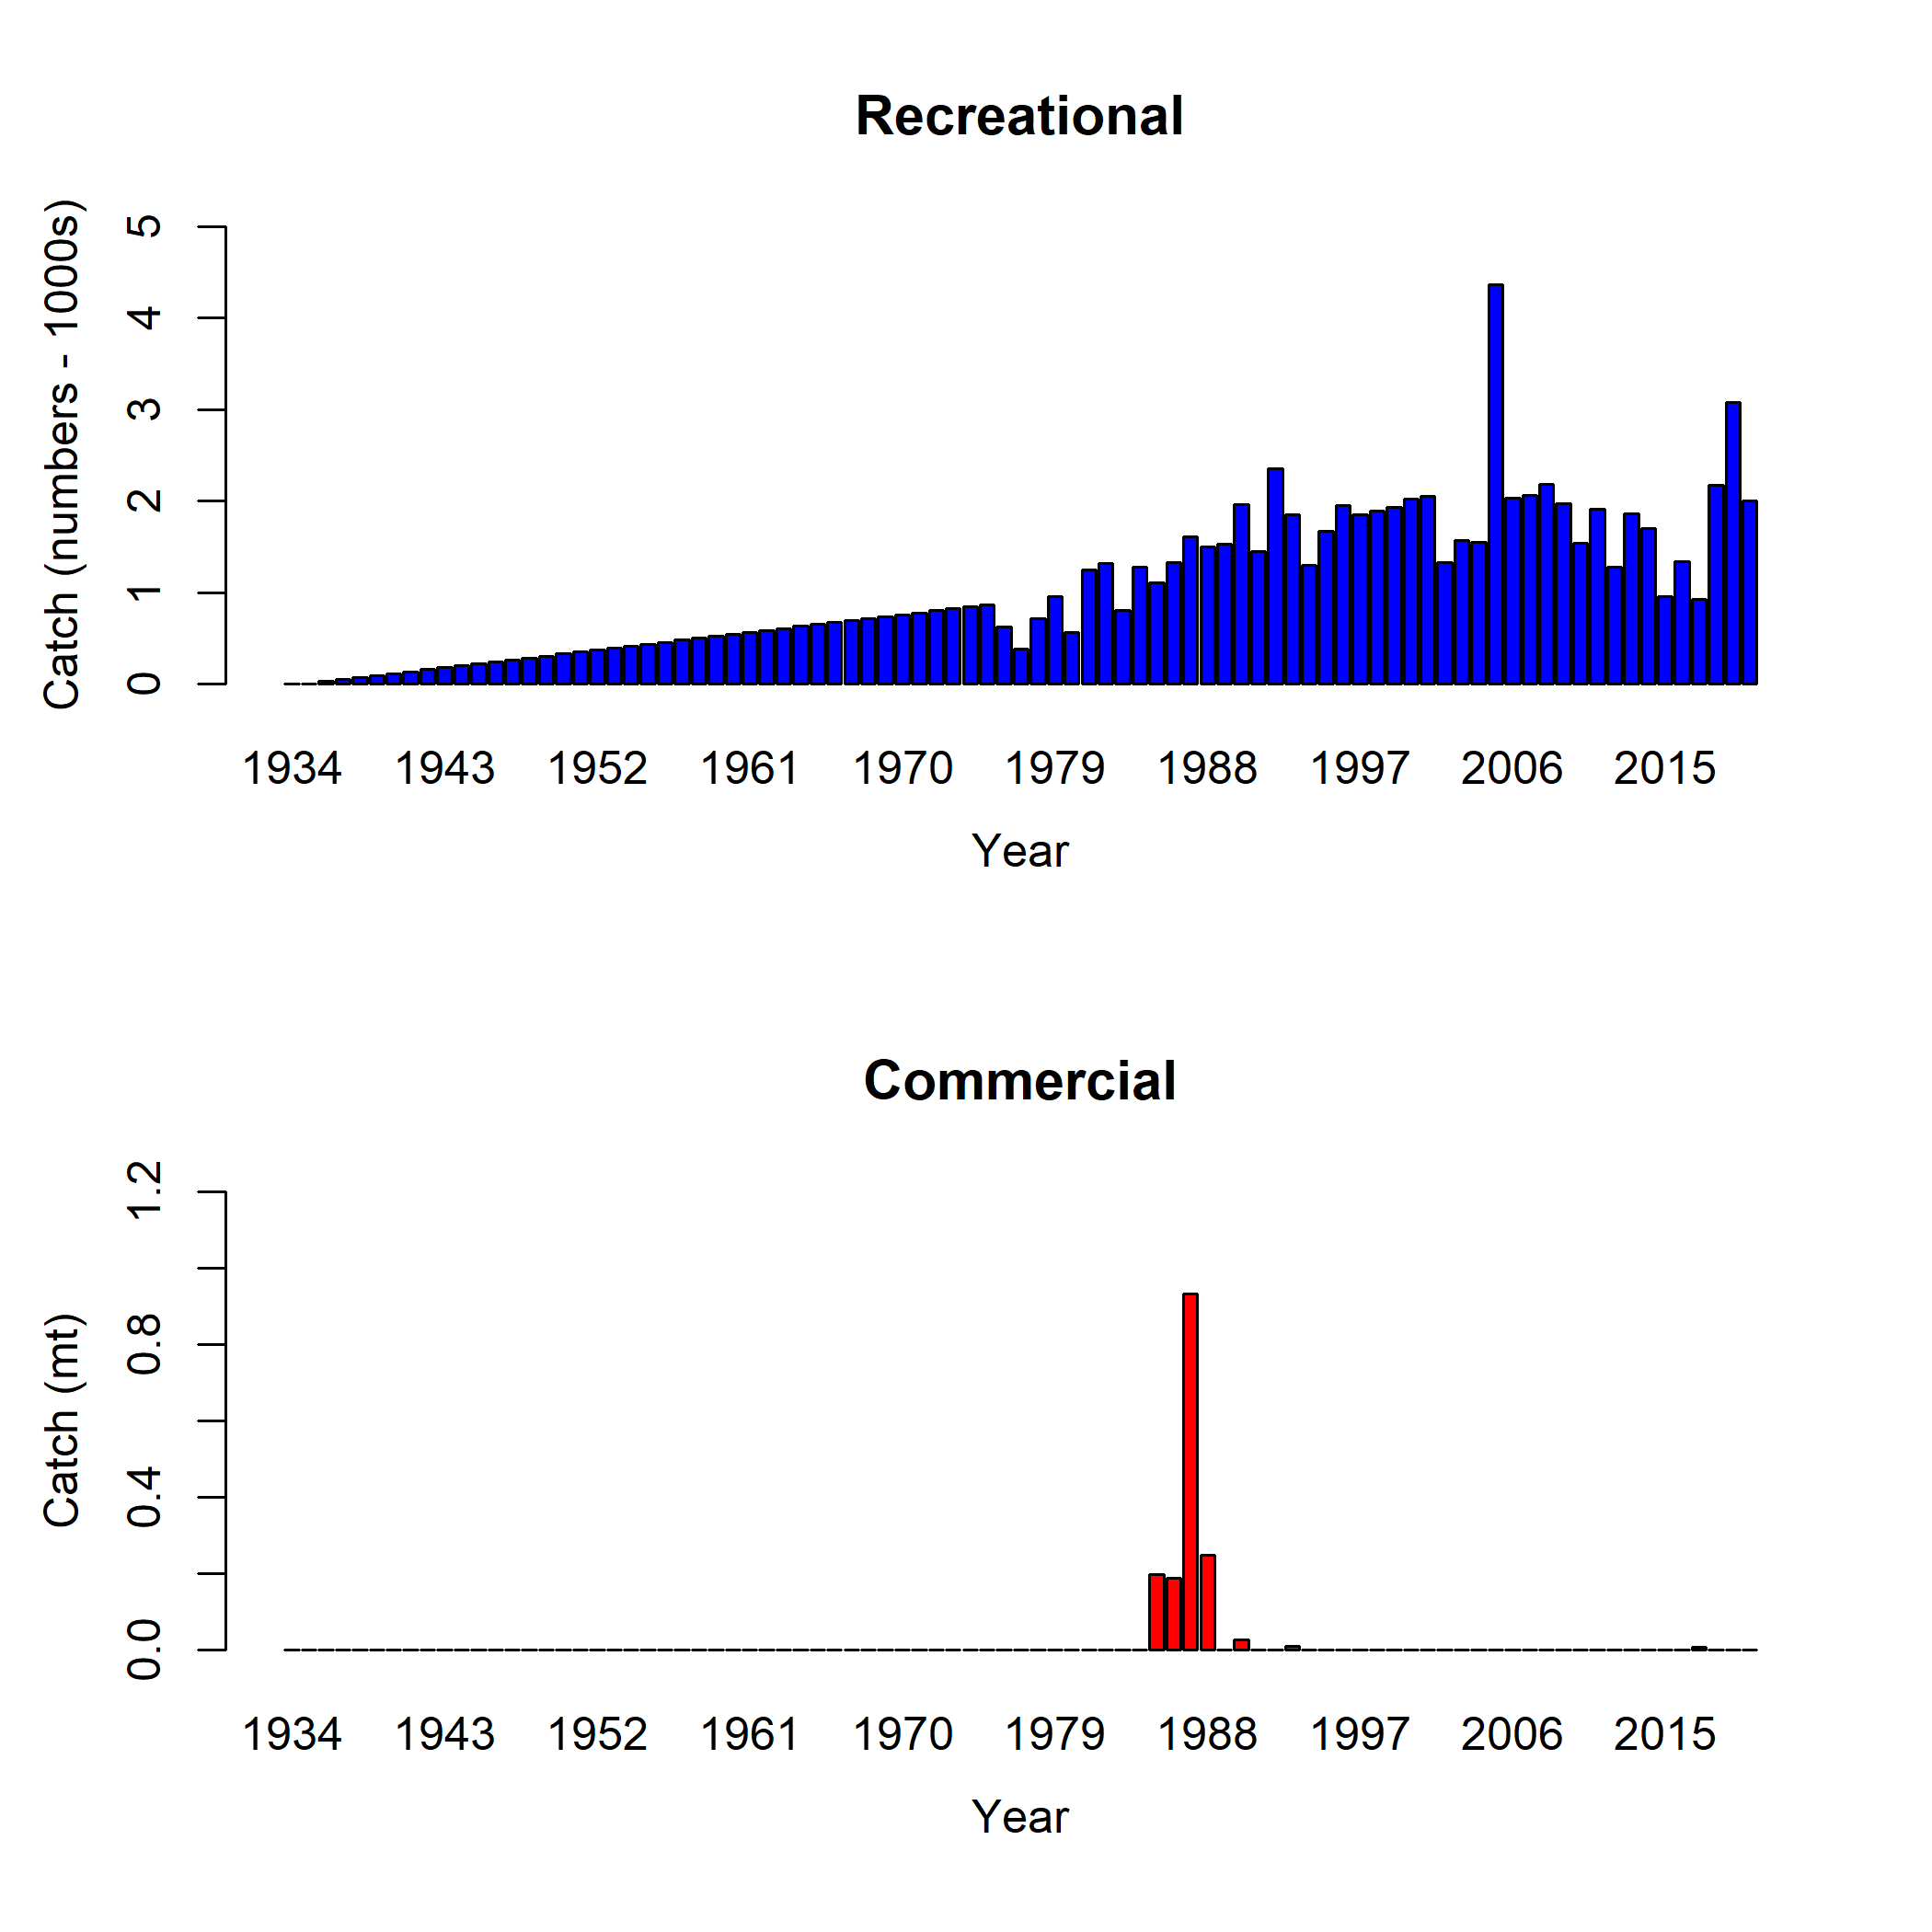
\includegraphics[width=1\textwidth,height=1\textheight]{figs/catches_wa.png}
\caption{Catches by year for the recreational and commercial fleets in the model.\label{fig:catch}}
\end{figure}

\tagmcend\tagstructend

\tagstructbegin{tag=Figure,alttext={Summary of data sources used in the base model.}}\tagmcbegin{tag=Figure}

\begin{figure}
\centering
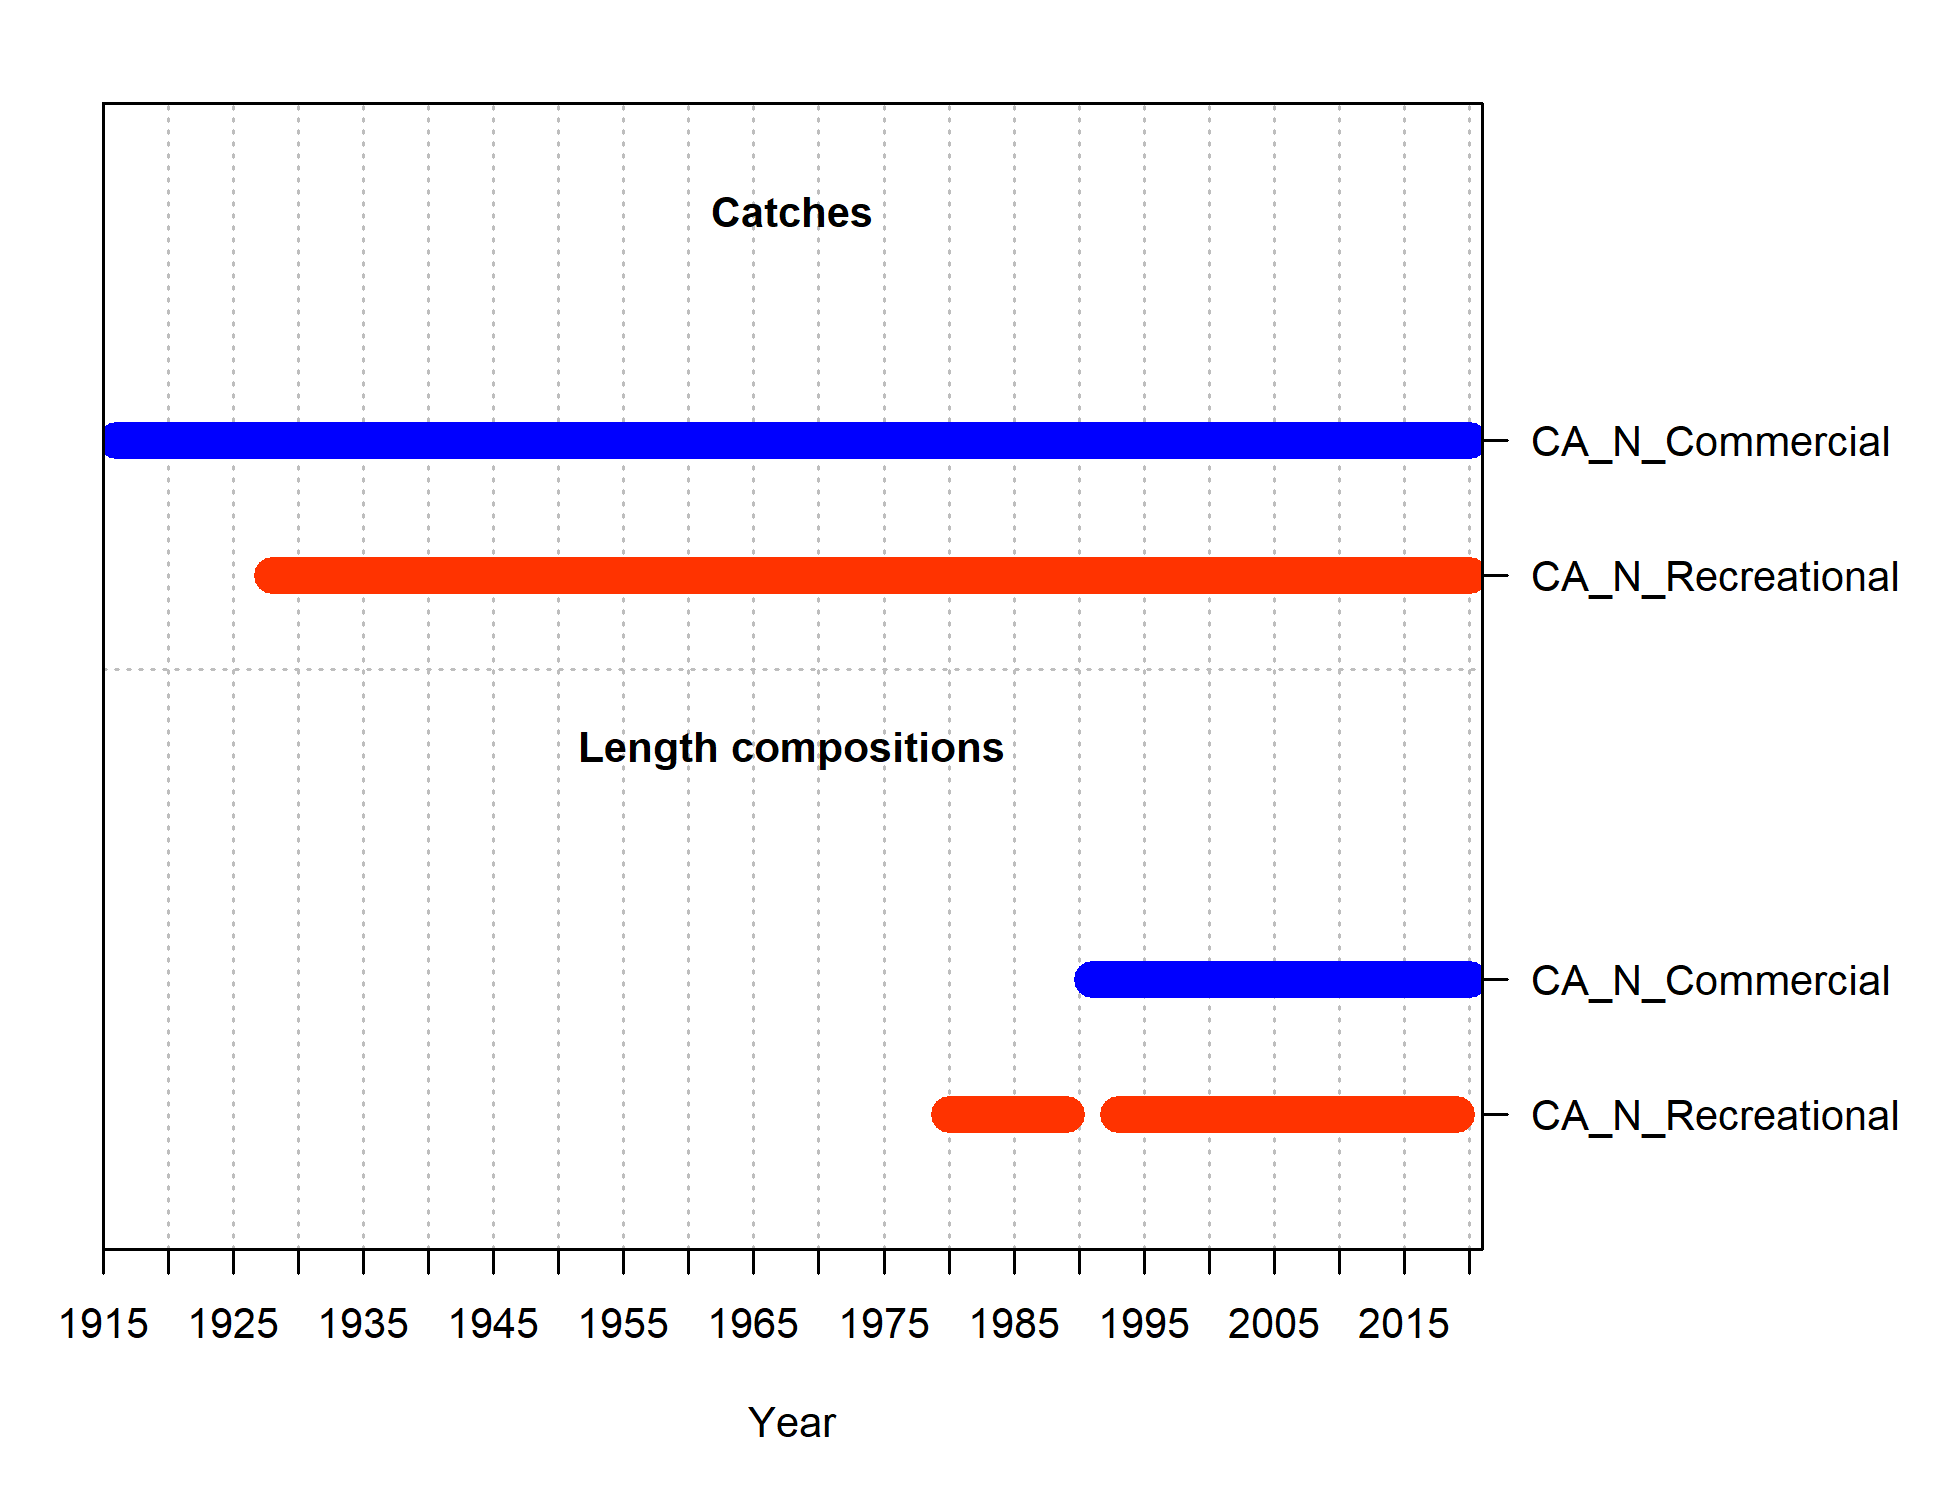
\includegraphics[width=1\textwidth,height=1\textheight]{C:/Assessments/2021/copper_rockfish_2021/models/wa/7.0_base/plots/data_plot.png}
\caption{Summary of data sources used in the base model.\label{fig:data-plot}}
\end{figure}

\tagmcend\tagstructend

\tagstructbegin{tag=Figure,alttext={Length composition data from the recreational fleet.}}\tagmcbegin{tag=Figure}

\begin{figure}
\centering
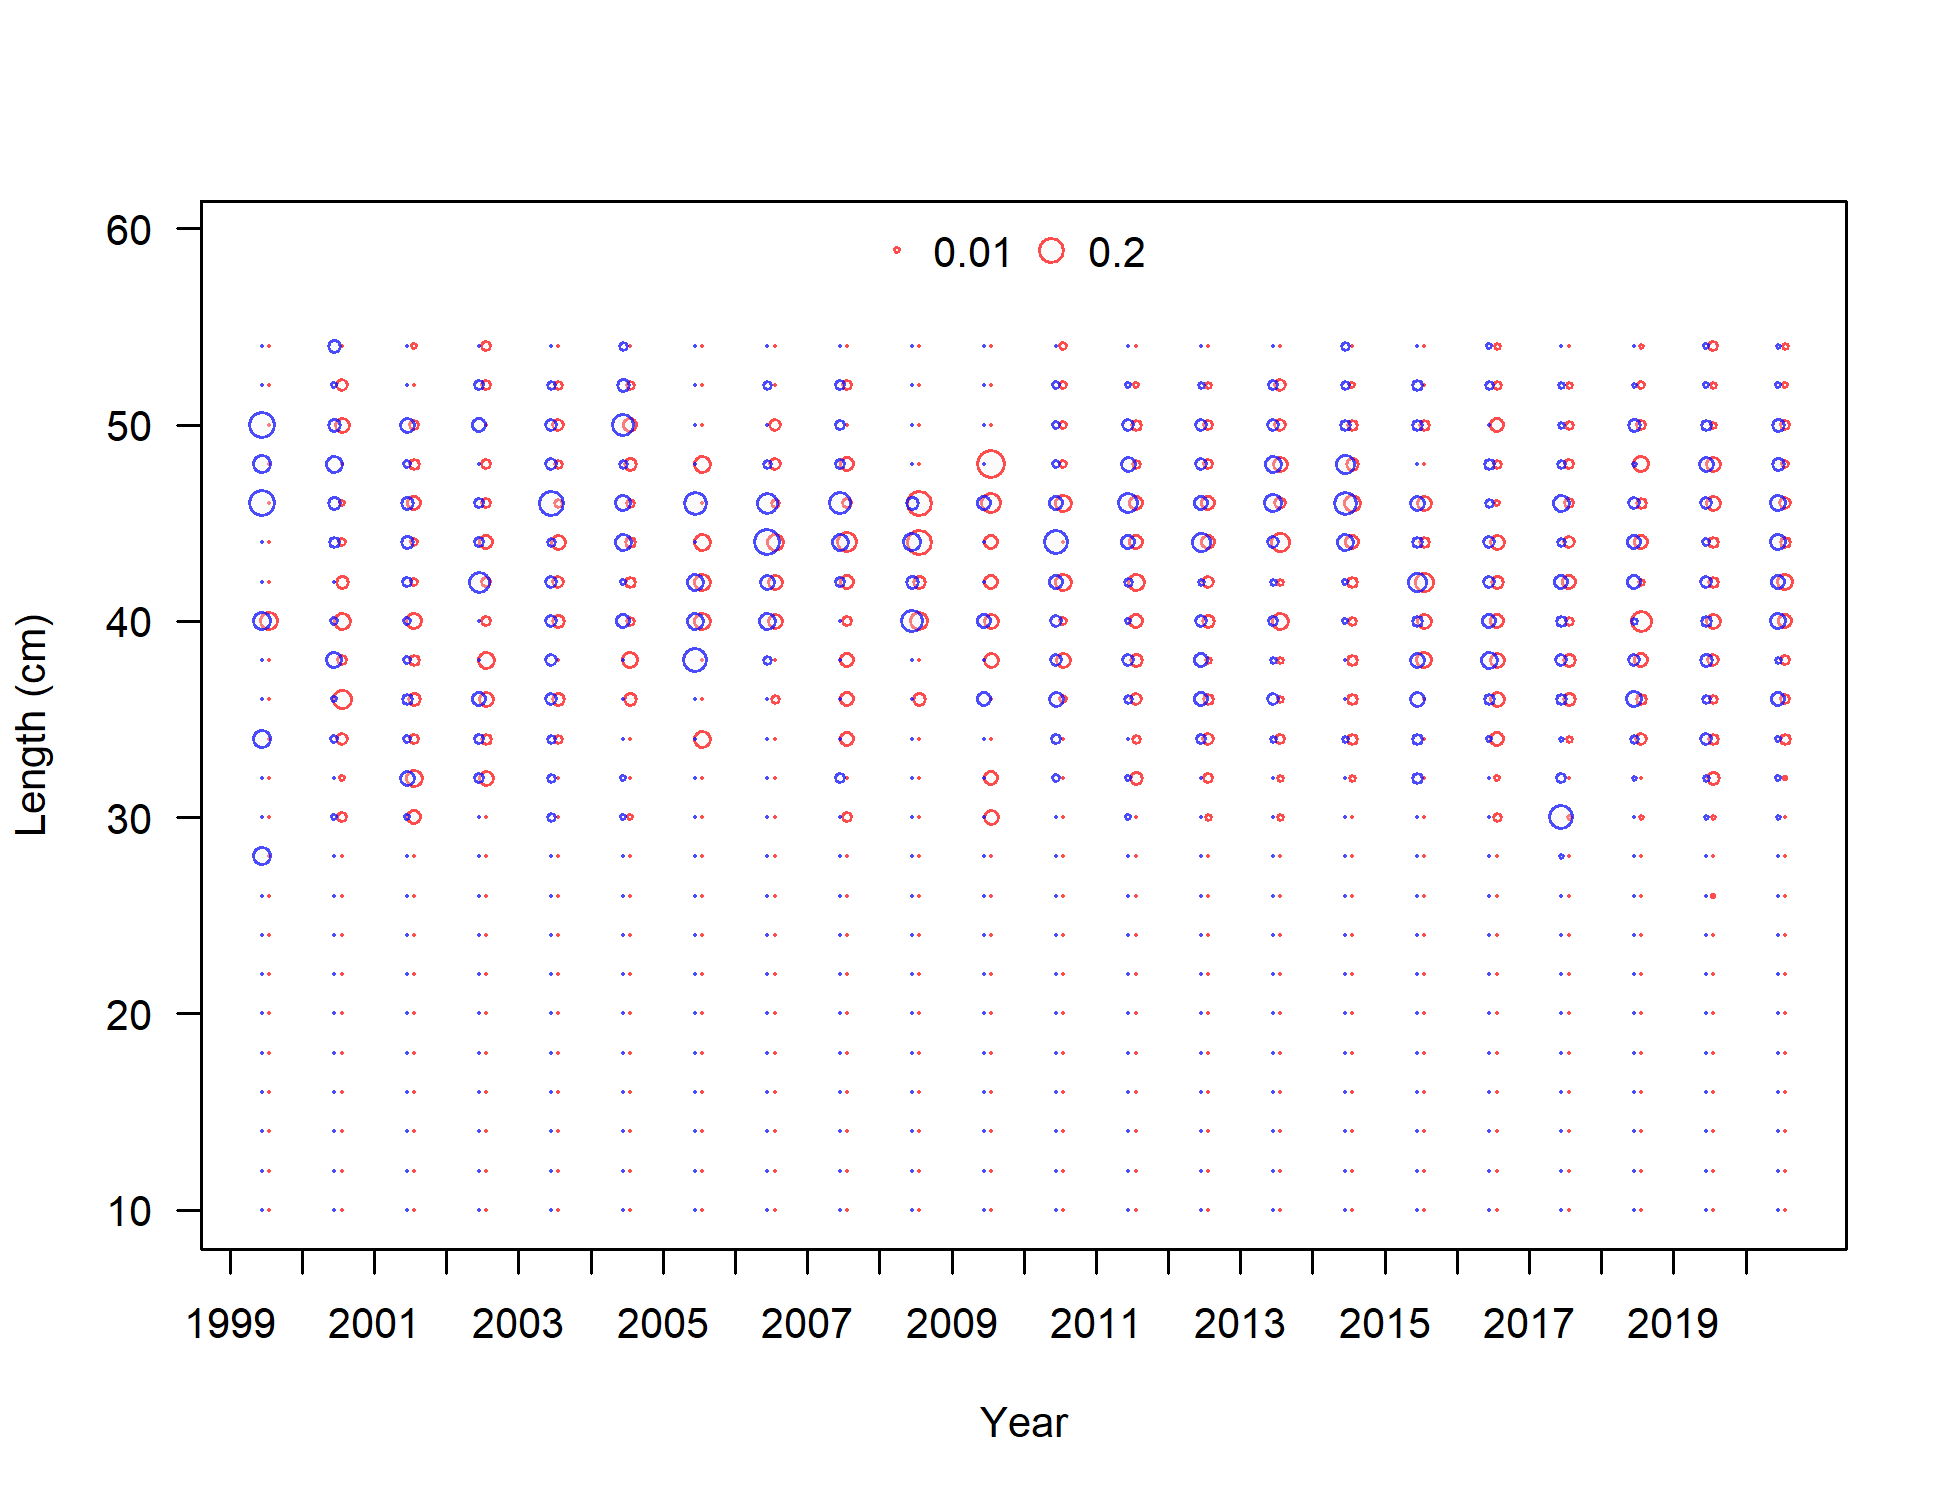
\includegraphics[width=1\textwidth,height=1\textheight]{C:/Assessments/2021/copper_rockfish_2021/models/wa/7.0_base/plots/comp_lendat_bubflt1mkt0_page2.png}
\caption{Length composition data from the recreational fleet.\label{fig:wa-len-data}}
\end{figure}

\tagmcend\tagstructend

\tagstructbegin{tag=Figure,alttext={Mean length for recreational fleet with 95 percent confidence intervals.}}\tagmcbegin{tag=Figure}

\begin{figure}
\centering
\includegraphics[width=1\textwidth,height=1\textheight]{C:/Assessments/2021/copper_rockfish_2021/models/wa/7.0_base/plots/comp_lendat_data_weighting_TA1.8_WA_Recreational.png}
\caption{Mean length for recreational fleet with 95 percent confidence intervals.\label{fig:mean-len-data}}
\end{figure}

\tagmcend\tagstructend

\tagstructbegin{tag=Figure,alttext={Comparison of the length-at-weight data from the NWFSC Hook and Line and the NWFSC WCGBT surveys.}}\tagmcbegin{tag=Figure}

\begin{figure}
\centering
\includegraphics[width=1\textwidth,height=1\textheight]{//nwcfile/FRAM/Assessments/CurrentAssessments/DataModerate_2021/copper_rockfish/data/biology/plots/doc_Length_Weight_Source.png}
\caption{Comparison of the length-at-weight data from the NWFSC Hook and Line and the NWFSC WCGBT surveys.\label{fig:len-weight-survey}}
\end{figure}

\tagmcend\tagstructend

\tagstructbegin{tag=Figure,alttext={Survey length-at-weight data with sex specific estimated fits.}}\tagmcbegin{tag=Figure}

\begin{figure}
\centering
\includegraphics[width=1\textwidth,height=1\textheight]{//nwcfile/FRAM/Assessments/CurrentAssessments/DataModerate_2021/copper_rockfish/data/biology/plots/doc_Length_Weight_Sex.png}
\caption{Survey length-at-weight data with sex specific estimated fits.\label{fig:len-weight}}
\end{figure}

\tagmcend\tagstructend

\tagstructbegin{tag=Figure,alttext={Observed length-at-age by data source.}}\tagmcbegin{tag=Figure}

\begin{figure}
\centering
\includegraphics[width=1\textwidth,height=1\textheight]{//nwcfile/FRAM/Assessments/CurrentAssessments/DataModerate_2021/copper_rockfish/data/biology/plots/doc_Data_Length_Age_by_Sex.png}
\caption{Observed length-at-age by data source.\label{fig:len-age-data}}
\end{figure}

\tagmcend\tagstructend

\tagstructbegin{tag=Figure,alttext={Length-at-age data from the with sex specific estimated growth.}}\tagmcbegin{tag=Figure}

\begin{figure}
\centering
\includegraphics[width=1\textwidth,height=1\textheight]{//nwcfile/FRAM/Assessments/CurrentAssessments/DataModerate_2021/copper_rockfish/data/biology/plots/doc_Length_Age_by_Sex.png}
\caption{Length-at-age data from the with sex specific estimated growth.\label{fig:len-age}}
\end{figure}

\tagmcend\tagstructend

\tagstructbegin{tag=Figure,alttext={Maturity as a function of  length.}}\tagmcbegin{tag=Figure}

\begin{figure}
\centering
\includegraphics[width=1\textwidth,height=1\textheight]{C:/Assessments/2021/copper_rockfish_2021/models/wa/7.0_base/plots/bio6_maturity.png}
\caption{Maturity as a function of length.\label{fig:maturity}}
\end{figure}

\tagmcend\tagstructend

\tagstructbegin{tag=Figure,alttext={Fecundity as a function of length.}}\tagmcbegin{tag=Figure}

\begin{figure}
\centering
\includegraphics[width=1\textwidth,height=1\textheight]{C:/Assessments/2021/copper_rockfish_2021/models/wa/7.0_base/plots/bio9_fecundity_len.png}
\caption{Fecundity as a function of length.\label{fig:fecundity}}
\end{figure}

\tagmcend\tagstructend

\tagstructbegin{tag=Figure,alttext={Fraction female by length across all available data sources.}}\tagmcbegin{tag=Figure}

\begin{figure}
\centering
\includegraphics[width=1\textwidth,height=1\textheight]{//nwcfile/FRAM/Assessments/CurrentAssessments/DataModerate_2021/copper_rockfish/data/biology/plots/Length_fraction_female.png}
\caption{Fraction female by length across all available data sources.\label{fig:len-sex-ratio}}
\end{figure}

\tagmcend\tagstructend

\tagstructbegin{tag=Figure,alttext={Fraction female by age across all available data sources.}}\tagmcbegin{tag=Figure}

\begin{figure}
\centering
\includegraphics[width=1\textwidth,height=1\textheight]{//nwcfile/FRAM/Assessments/CurrentAssessments/DataModerate_2021/copper_rockfish/data/biology/plots/Age_fraction_female.png}
\caption{Fraction female by age across all available data sources.\label{fig:age-sex-ratio}}
\end{figure}

\tagmcend\tagstructend

\tagstructbegin{tag=Figure,alttext={Selectivity at length by fleet.}}\tagmcbegin{tag=Figure}

\begin{figure}
\centering
\includegraphics[width=1\textwidth,height=1\textheight]{C:/Assessments/2021/copper_rockfish_2021/models/wa/7.0_base/plots/sel01_multiple_fleets_length1.png}
\caption{Selectivity at length by fleet.\label{fig:selex}}
\end{figure}

\tagmcend\tagstructend

\tagstructbegin{tag=Figure,alttext={Estimated time series of age-0 recruits (1000s).}}\tagmcbegin{tag=Figure}

\begin{figure}
\centering
\includegraphics[width=1\textwidth,height=1\textheight]{C:/Assessments/2021/copper_rockfish_2021/models/wa/7.0_base/plots/ts11_Age-0_recruits_(1000s)_with_95_asymptotic_intervals.png}
\caption{Estimated time series of age-0 recruits (1000s).\label{fig:recruits}}
\end{figure}

\tagmcend\tagstructend

\tagstructbegin{tag=Figure,alttext={Length at age in the beginning of the year in the ending year of the model.}}\tagmcbegin{tag=Figure}

\begin{figure}
\centering
\includegraphics[width=1\textwidth,height=1\textheight]{C:/Assessments/2021/copper_rockfish_2021/models/wa/7.0_base/plots/bio1_sizeatage.png}
\caption{Length at age in the beginning of the year in the ending year of the model.\label{fig:len-age-ss}}
\end{figure}

\tagmcend\tagstructend

\tagstructbegin{tag=Figure,alttext={Pearson residuals for recreational fleet. Closed bubble are positive residuals (observed > expected) and open bubbles are negative residuals (observed < expected).}}\tagmcbegin{tag=Figure}

\begin{figure}
\centering
\includegraphics[width=1\textwidth,height=1\textheight]{C:/Assessments/2021/copper_rockfish_2021/models/wa/7.0_base/plots/comp_lenfit_residsflt1mkt0_page2.png}
\caption{Pearson residuals for recreational fleet. Closed bubble are positive residuals (observed \textgreater{} expected) and open bubbles are negative residuals (observed \textless{} expected).\label{fig:rec-pearson}}
\end{figure}

\tagmcend\tagstructend

\tagstructbegin{tag=Figure,alttext={Mean length for recreational with 95 percent confidence intervals based on current samples sizes.}}\tagmcbegin{tag=Figure}

\begin{figure}
\centering
\includegraphics[width=1\textwidth,height=1\textheight]{C:/Assessments/2021/copper_rockfish_2021/models/wa/7.0_base/plots/comp_lenfit_data_weighting_TA1.8_WA_Recreational.png}
\caption{Mean length for recreational with 95 percent confidence intervals based on current samples sizes.\label{fig:rec-mean-len-fit}}
\end{figure}

\tagmcend\tagstructend

\tagstructbegin{tag=Figure,alttext={Aggregated length comps over all years.}}\tagmcbegin{tag=Figure}

\begin{figure}
\centering
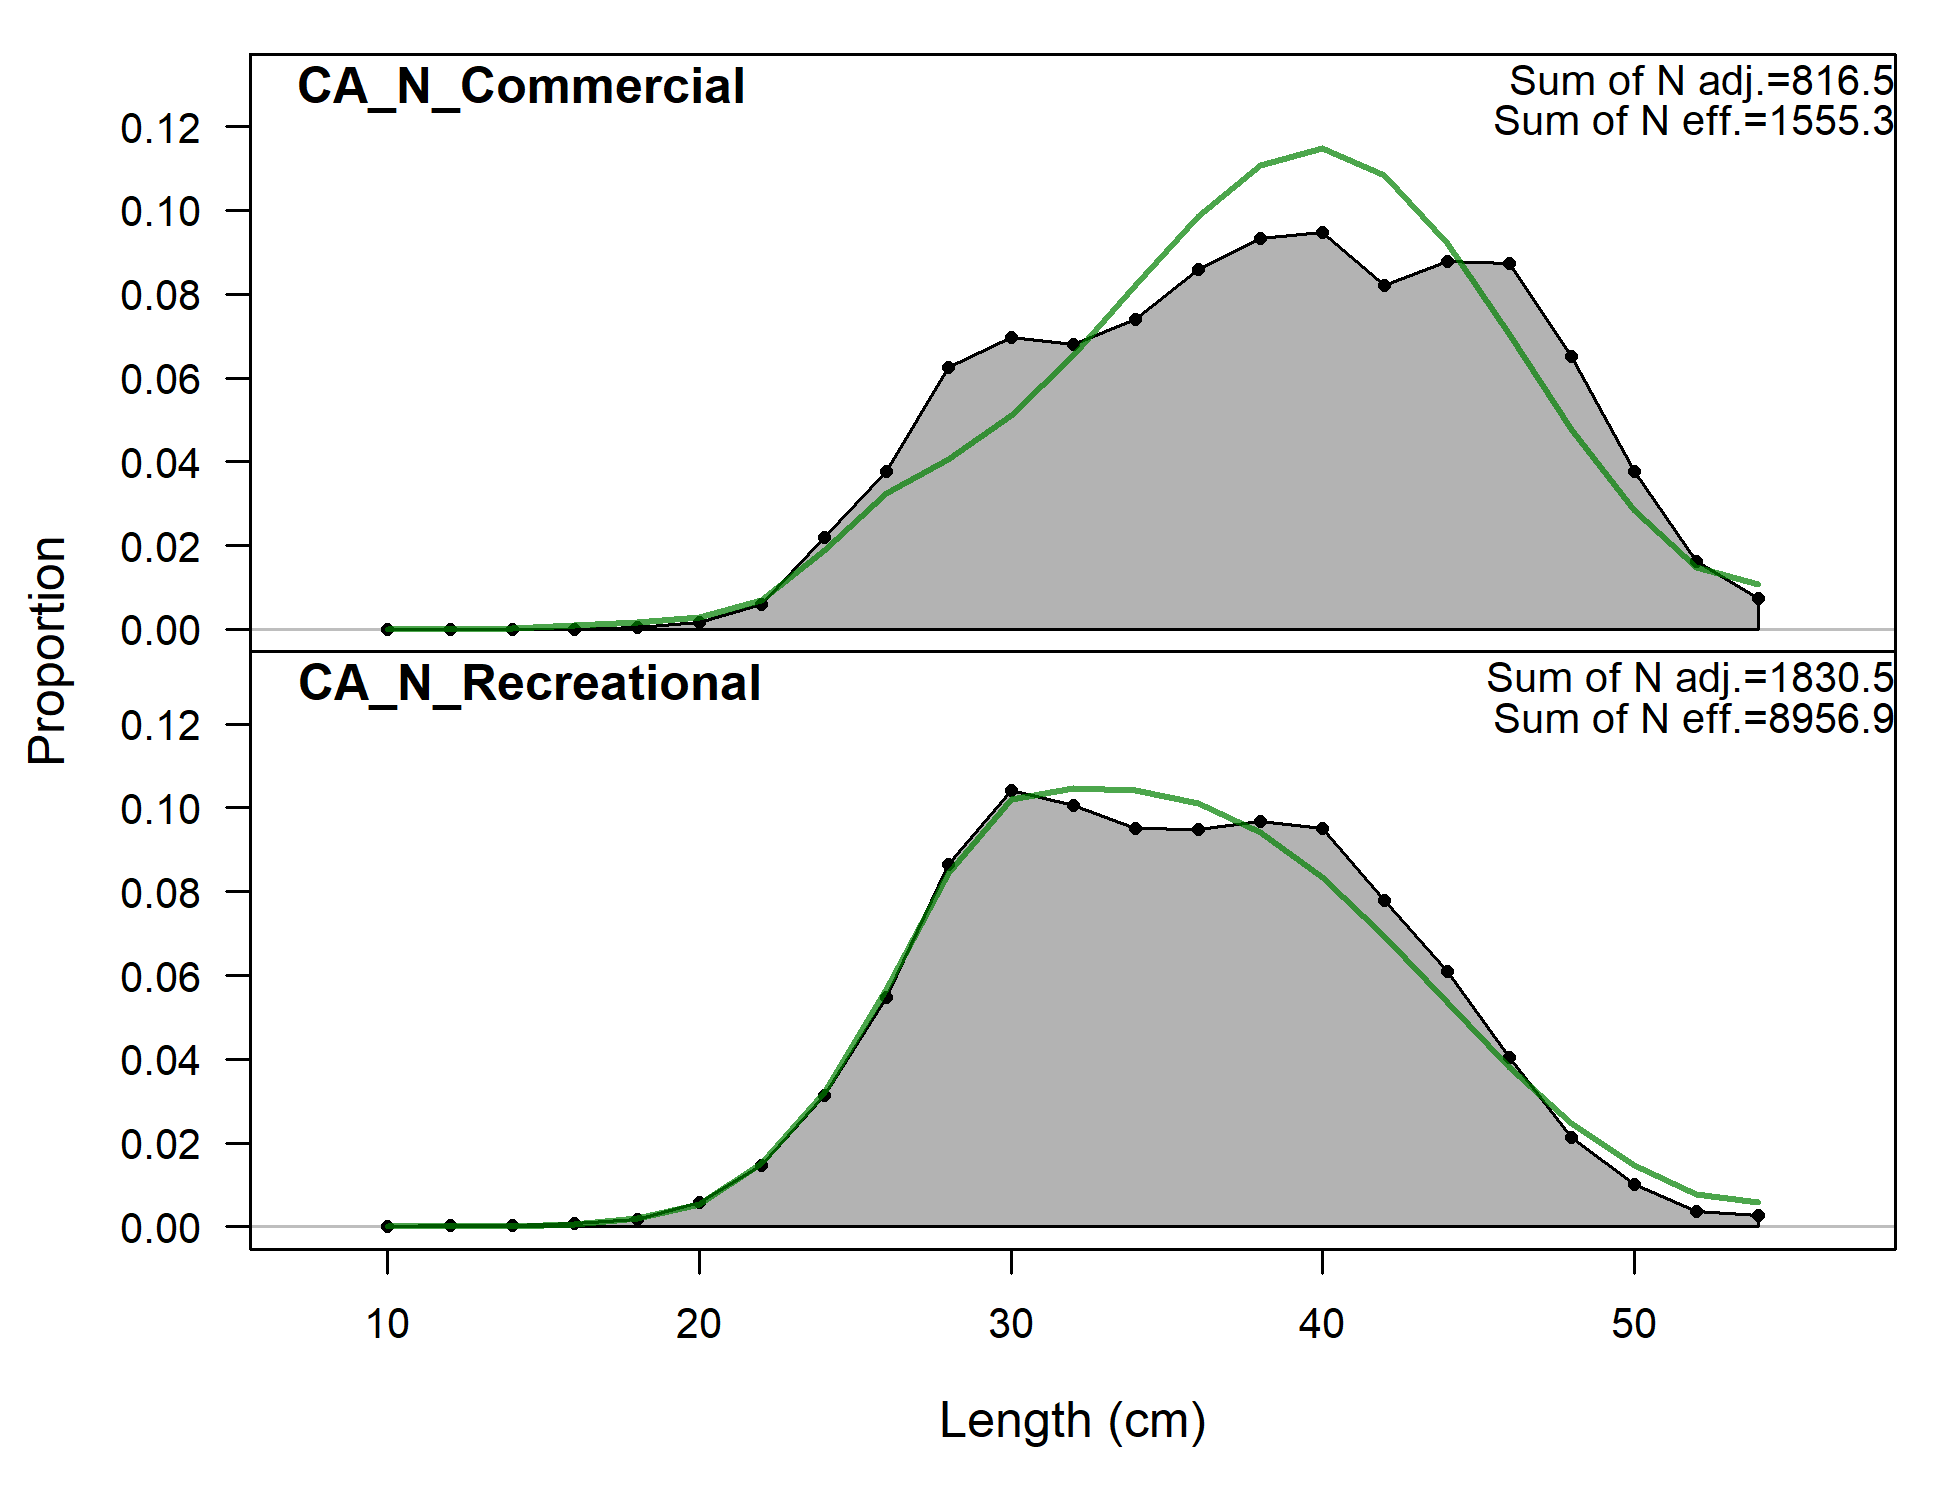
\includegraphics[width=1\textwidth,height=1\textheight]{C:/Assessments/2021/copper_rockfish_2021/models/wa/7.0_base/plots/comp_lenfit__aggregated_across_time.png}
\caption{Aggregated length comps over all years.\label{fig:agg-len-fit}}
\end{figure}

\tagmcend\tagstructend

\tagstructbegin{tag=Figure,alttext={Estimated time series of spawning output.}}\tagmcbegin{tag=Figure}

\begin{figure}
\centering
\includegraphics[width=1\textwidth,height=1\textheight]{C:/Assessments/2021/copper_rockfish_2021/models/wa/7.0_base/plots/ts7_Spawning_output_with_95_asymptotic_intervals_intervals.png}
\caption{Estimated time series of spawning output.\label{fig:ssb}}
\end{figure}

\tagmcend\tagstructend

\tagstructbegin{tag=Figure,alttext={Estimated time series of total biomass.}}\tagmcbegin{tag=Figure}

\begin{figure}
\centering
\includegraphics[width=1\textwidth,height=1\textheight]{C:/Assessments/2021/copper_rockfish_2021/models/wa/7.0_base/plots/ts1_Total_biomass_(mt).png}
\caption{Estimated time series of total biomass.\label{fig:tot-bio}}
\end{figure}

\tagmcend\tagstructend

\tagstructbegin{tag=Figure,alttext={Estimated time series of fraction of unfished spawning output.}}\tagmcbegin{tag=Figure}

\begin{figure}
\centering
\includegraphics[width=1\textwidth,height=1\textheight]{C:/Assessments/2021/copper_rockfish_2021/models/wa/7.0_base/plots/ts9_Fraction_of_unfished_with_95_asymptotic_intervals_intervals.png}
\caption{Estimated time series of fraction of unfished spawning output.\label{fig:depl}}
\end{figure}

\tagmcend\tagstructend

\tagstructbegin{tag=Figure,alttext={Stock-recruit curve. Point colors indicate year, with warmer colors indicating earlier years and cooler colors in showing later years.}}\tagmcbegin{tag=Figure}

\begin{figure}
\centering
\includegraphics[width=1\textwidth,height=1\textheight]{C:/Assessments/2021/copper_rockfish_2021/models/wa/7.0_base/plots/SR_curve.png}
\caption{Stock-recruit curve. Point colors indicate year, with warmer colors indicating earlier years and cooler colors in showing later years.\label{fig:bh-curve}}
\end{figure}

\tagmcend\tagstructend

\tagstructbegin{tag=Figure,alttext={Estimated 1 - relative spawning ratio (SPR) by year.}}\tagmcbegin{tag=Figure}

\begin{figure}
\centering
\includegraphics[width=1\textwidth,height=1\textheight]{C:/Assessments/2021/copper_rockfish_2021/models/wa/7.0_base/plots/SPR2_minusSPRseries.png}
\caption{Estimated 1 - relative spawning ratio (SPR) by year.\label{fig:1-spr}}
\end{figure}

\tagmcend\tagstructend

\tagstructbegin{tag=Figure,alttext={Equilibrium yield curve for the base case model. Values are based on the 2020 fishery selectivity and with steepness fixed at 0.72.}}\tagmcbegin{tag=Figure}

\begin{figure}
\centering
\includegraphics[width=1\textwidth,height=1\textheight]{C:/Assessments/2021/copper_rockfish_2021/models/wa/7.0_base/plots/yield2_yield_curve_with_refpoints.png}
\caption{Equilibrium yield curve for the base case model. Values are based on the 2020 fishery selectivity and with steepness fixed at 0.72.\label{fig:yield}}
\end{figure}

\tagmcend\tagstructend

\clearpage

\tagstructbegin{tag=H1}\tagmcbegin{tag=H1}

\hypertarget{references}{%
\section{References}\label{references}}

\leavevmode\tagmcend\tagstructend

\hypertarget{refs}{}
\begin{cslreferences}
\leavevmode\hypertarget{ref-bizzarro_diet_2017-1}{}%
Bizzarro, Joseph J., Mary M. Yoklavich, and W. Waldo Wakefield. 2017. ``Diet Composition and Foraging Ecology of U.S. Pacific Coast Groundfishes with Applications for Fisheries Management.'' \emph{Environmental Biology of Fishes} 100 (4): 375--93. \url{https://doi.org/10.1007/s10641-016-0529-2}.

\leavevmode\hypertarget{ref-buonaccorsi_population_2002}{}%
Buonaccorsi, Vincent P, Carol A Kimbrell, Eric A Lynn, and Russell D Vetter. 2002. ``Population Structure of Copper Rockfish ( \emph{Sebastes Caurinus} ) Reflects Postglacial Colonization and Contemporary Patterns of Larval Dispersal.'' \emph{Canadian Journal of Fisheries and Aquatic Sciences} 59 (8): 1374--84. \url{https://doi.org/10.1139/f02-101}.

\leavevmode\hypertarget{ref-cope_data-moderate_2013}{}%
Cope, Jason, E. J. Dick, Alec MacCall, Melissa Monk, Braden Soper, and Chantel Wetzel. 2013. ``Data-Moderate Stock Assessments for Brown, China, Copper, Sharpchin, Stripetail, and Yellowtail Rockfishes and English and Rex Soles in 2013.'' 7700 Ambassador Place NE, Suite 200, Portland, OR: Pacific Fishery Management Council. \url{http://www.academia.edu/download/44999856/CopeetalDataModerate2013.pdf}.

\leavevmode\hypertarget{ref-cope_approach_2011}{}%
Cope, Jason M., John DeVore, E. J. Dick, Kelly Ames, John Budrick, Daniel L. Erickson, Joanna Grebel, et al. 2011. ``An Approach to Defining Stock Complexes for U.S. West Coast Groundfishes Using Vulnerabilities and Ecological Distributions.'' \emph{North American Journal of Fisheries Management} 31 (4): 589--604. \url{https://doi.org/10.1080/02755947.2011.591264}.

\leavevmode\hypertarget{ref-dick_meta-analysis_2017}{}%
Dick, E. J., Sabrina Beyer, Marc Mangel, and Stephen Ralston. 2017. ``A Meta-Analysis of Fecundity in Rockfishes (Genus \emph{Sebastes}).'' \emph{Fisheries Research} 187 (March): 73--85. \url{https://doi.org/10.1016/j.fishres.2016.11.009}.

\leavevmode\hypertarget{ref-dick_replicate_2014}{}%
Dick, S., J. B. Shurin, and E. B. Taylor. 2014. ``Replicate Divergence Between and Within Sounds in a Marine Fish: The Copper Rockfish ( \emph{Sebastes Caurinus} ).'' \emph{Molecular Ecology} 23 (3): 575--90. \url{https://doi.org/10.1111/mec.12630}.

\leavevmode\hypertarget{ref-francis_data_2011}{}%
Francis, R. I. C. Chris, and Ray Hilborn. 2011. ``Data Weighting in Statistical Fisheries Stock Assessment Models.'' \emph{Canadian Journal of Fisheries and Aquatic Sciences} 68 (6): 1124--38. \url{https://doi.org/10.1139/f2011-025}.

\leavevmode\hypertarget{ref-hamel_method_2015}{}%
Hamel, Owen S. 2015. ``A Method for Calculating a Meta-Analytical Prior for the Natural Mortality Rate Using Multiple Life History Correlates.'' \emph{ICES Journal of Marine Science: Journal Du Conseil} 72 (1): 62--69. \url{https://doi.org/10.1093/icesjms/fsu131}.

\leavevmode\hypertarget{ref-hannah_length_2014}{}%
Hannah, Robert W. 2014. ``Length and Age at Maturity of Female Copper Rockfish (\emph{Sebastes Caurinus}) from Oregon Waters Based on Histological Evaluation of Ovaries.'' Information Reports 2014-04. Oregon Department of Fish; Wildlife.

\leavevmode\hypertarget{ref-johansson_influence_2008}{}%
Johansson, M. L., M. A. Banks, K. D. Glunt, H. M. Hassel-Finnegan, and V. P. Buonaccorsi. 2008. ``Influence of Habitat Discontinuity, Geographical Distance, and Oceanography on Fine-Scale Population Genetic Structure of Copper Rockfish ( \emph{Sebastes Caurinus} ).'' \emph{Molecular Ecology} 17 (13): 3051--61. \url{https://doi.org/10.1111/j.1365-294X.2008.03814.x}.

\leavevmode\hypertarget{ref-lea_biological_1999}{}%
Lea, Robert N, Robert D McAllister, and David A VenTresca. 1999. ``Biological Sspects of Nearshore Rockfishes of the Genus Sebastes from Central California with Notes on Ecologically Related Sport Fishes.'' Fish Bulletin 177. State of California The Resources Agency Department of Fish; Game.

\leavevmode\hypertarget{ref-love_milton_probably_1996}{}%
Love, Milton. 1996. \emph{Probably More Than You Want to Know About the Fishes of the Pacific Coast}. Santa Barbara, California: Really Big Press.

\leavevmode\hypertarget{ref-mcallister_bayesian_1997}{}%
McAllister, M. K., and J. N. Ianelli. 1997. ``Bayesian Stock Assessment Using Catch-Age Data and the Sampling - Importance Resampling Algorithm.'' \emph{Canadian Journal of Fisheries and Aquatic Sciences} 54: 284--300.

\leavevmode\hypertarget{ref-miller_guide_1972}{}%
Miller, Daniel J, and Robert N Lea. 1972. ``Guide to Coastal Marine Fishes of California.'' Fish Bulletin 157. State of California Department of Fish; Game Bureau of Marine Fisheries.

\leavevmode\hypertarget{ref-ralston_documentation_2010}{}%
Ralston, Stephen, Don E. Pearson, John C. Field, and Meisha Key. 2010. ``Documentation of the California Catch Reconstruction Project.'' US Department of Commerce, National Oceanic; Atmospheric Adminstration, National Marine.

\leavevmode\hypertarget{ref-sivasundar_life_2010}{}%
Sivasundar, Arjun, and Stephen R. Palumbi. 2010. ``Life History, Ecology and the Biogeography of Strong Genetic Breaks Among 15 Species of Pacific Rockfish, Sebastes.'' \emph{Marine Biology} 157 (7): 1433--52. \url{https://doi.org/10.1007/s00227-010-1419-3}.

\leavevmode\hypertarget{ref-then_evaluating_2015-1}{}%
Then, A. Y., J. M. Hoenig, N. G. Hall, and D. A. Hewitt. 2015. ``Evaluating the Predictive Performance of Empirical Estimators of Natural Mortality Rate Using Information on over 200 Fish Species.'' \emph{ICES Journal of Marine Science} 72 (1): 82--92. \url{https://doi.org/10.1093/icesjms/fsu136}.

\leavevmode\hypertarget{ref-thorson_model-based_2017}{}%
Thorson, James T., Kelli F. Johnson, Richard D. Methot, and Ian G. Taylor. 2017. ``Model-Based Estimates of Effective Sample Size in Stock Assessment Models Using the Dirichlet-Multinomial Distribution.'' \emph{Fisheries Research} 192: 84--93. \url{https://doi.org/10.1016/j.fishres.2016.06.005}.
\end{cslreferences}
\end{document}
